%%
%% This is file `example.tex',
%% generated with the docstrip utility.
%%
%% The original source files were:
%%
%% drexel-thesis.dtx  (with options: `example')
%% 
%% This is a generated file.
%% 
%% Copyright (C) 2010 W. Trevor King
%% 
%% This file may be distributed and/or modified under the conditions of
%% the LaTeX Project Public License, either version 1.3 of this license
%% or (at your option) any later version.  The latest version of this
%% license is in:
%% 
%%    http://www.latex-project.org/lppl.txt
%% 
%% and version 1.3 or later is part of all distributions of LaTeX version
%% 2003/06/01 or later.
%% 
%% See drexel-thesis.pdf for details.
\documentclass[subfig,blackref,approvalform]{drexel-thesis}

%% Enter the appropriate information here
\author{Hunter Kippen}
\title{A New Approach to Detecting Frame Deletion in H.264 Encoded Digital Video}
\DUTmonth{May}
\DUTyear{2019}
\degree{Master of Science}
\advisor{Dr. Matthew Stamm, Ph.D.}
\copyrighttext{\copyrighttextCCBYSA}

%\usepackage[super,sort&compress]{natbib} % fancy citation extensions
%\bibliographystyle{IEEE}

\usepackage[backend=bibtex,style=ieee,natbib=true]{biblatex}
\addbibresource{references.bib}

\usepackage{fancyvrb} % nicer verbatim handling
\DefineShortVerb{\|}  % \verb+TEXT+  ->  |TEXT|

\renewenvironment{preamble}{% look, we're clobbering an environment!
  What preamble?\begingroup\color{white}}{\endgroup}

\usepackage[english]{babel} % English blindtext
\usepackage{blindtext} % macros for producing dummy output
\usepackage{amsmath}
\usepackage{amssymb}
\usepackage{dsfont}
\usepackage{bm}
\usepackage{subfig}
\usepackage{wrapfig}
\usepackage{tabu}
\usepackage{adjustbox}

\DeclareMathOperator*{\argmin}{argmin}
\DeclareMathOperator*{\R}{\mathbb{R}}

\addto\captionsenglish{\DUTnames}

\begin{document}
\begin{DUTpreamble} % "DUT" because original preamble was clobbered.

%\begin{dedications}
%\Blindtext[3]
%\end{dedications}

%\begin{acknowledgments}
%\Blindtext[3]
%\end{acknowledgments}

\tableofcontents
\listoftables
\listoffigures

\begin{abstract}

Due to the increasing prevalence of falsified video content, it is important to be able to identify altered video recordings. For certain types of video, removing small portions of content can change the perception of the events that transpire without leaving visually detectable evidence. In particular, removing a set or sequence of frames from the beginning of a video can change the context of surrounding events, especially in newsworthy content. Digital forensic techniques have been developed to detect this type of video manipulation, but were originally proposed for use on MPEG-2 video. Advances in video encoding, particularly in MPEG-4 and H.264 have called the effectiveness of these techniques into question. In this thesis, we examine the performance of detectors built using the methodology from MPEG-2 when applied to H.264 video, and show that indeed new methods are needed to detect frame deletion in modern video. We propose a new method for extracting fingerprints left behind by frame deletion in H.264 as well as an expanded frame deletion detection framework for ensuring robustness across videos captured by different camera models as well as variation in scene content or motion. We evaluate the performance of our proposed techniques as well as examine current limitations.

\end{abstract}
\end{DUTpreamble}

\begin{thesis}
% This file is for the Introduction section of the Master's Thesis.
% This file will not compile on it's own. Will need to include it into a main file
% That uses the drexel thesis template.
\chapter{Introduction}

In recent years, due to the increasing ease by which an individual is able to alter or falsify digital image content, video recordings have supplanted images as evidence that events have occurred. The proliferation of smartphones has made video recording accessible to a large portion of the population. However, it has become increasingly apparent that video evidence is not foolproof. Falsified video content is increasingly being disseminated to the general populace, often from sources they trust. To combat this, research into digital media forensics has emerged over the past 15 years.

Digital media forensics seeks to provide information about digital media without the use of information that is not intrinsic to the piece of media in question. Specifically, digital media forensic techniques are formulated to work without the use of metadata or implanted watermarks to make a determination about the nature of digital media content. As such, the techniques instead process the multimedia content to extract fingerprints, which are specific signals left in media content by editing operations or the media capture process. These forensic techniques have become incredibly important in verifying the legitimacy of digital media content.

Research into digital media forensics has been developed to solve a wide variety of forensics problems. One well studied problem is that of source identification. Given a sample of digital media, can an investigator figure out the source of the content? In this particular case, source can mean what individual or group captured the specific piece of content or what hardware was used to capture the content. For visual media, research has largely been focused on what device or Make and model was used to capture content. Image source identification research has not only been able to determine what model of camera captured an image \cite{imagesourceid}, but also what specific device \cite{prnu} has captured an image. Recent work has been conducted on determining the source camera model of video content as well \cite{videosourceid}.

Another significant problem studied by digital media forensics researchers is that of media forgery detection. Given a sample of digital media, can an investigator determine the authenticity of the content? Has the image or video undergone additional post-processing after it was captured, and does this post processing affect the perception of the content? There are many different editing operations that can be done on images, each of which introduces different fingerprints that can be detected. Detecting contrast enhancement \cite{contrastenhance}, resampling \cite{resampling}, double compression \cite{doubleJPEG}, and others \cite{lca} can help an investigator determine an image's processing history, and make a determination as to the authenticity of the content.

Detecting forgery in video is a much more difficult task. As a video consists of multiple images, often of lower quality due to heavy compression, fingerprints are more difficult to extract. One particular video editing operation that has seen significant research is that of video frame deletion. Video frame deletion occurs when a frame or sequence of frames is removed from a video. To do this, a forger must decode the video, remove a frame or sequence of frames, then reencode the video. If frames are removed from the beginning of a video sequence, a forger can produce a video that has no discernible difference between a freshly captured video but can portray a significantly different message to a viewer. An example of this is in video of violent protests or police brutality. If there are inciting incidents to the violence, removing the context surrounding the events can make otherwise justified actions seem unreasonable.

To date, most techniques to detect video frame deletion were formulated to work on MPEG-2 encoded video\cite{wang} \cite{stamm}. The techniques largely rely on traces left by the video frame prediction process. Most video encoding standards define a procedure for predicting the image content in a frame from other frames in the video. This is known as inter-frame prediction. Inter-frame prediction is crucial to improving compression rates with minimal perceptible loss in visual quality. Modern video codecs such as H.264 or MPEG-4 contain more advanced techniques used in the frame prediction process. Thus, it is not clear whether the traces used to detect frame deletion on MPEG-2 are expressed in modern video. 

In this thesis, we show that indeed the advances in video encoding disrupt the traces left by frame deletion. Thus we propose a new technique for extracting the frame deletion traces for use on modern video codecs. In addition, we propose using added features and an autoregressive (AR) model to capture statistical variations between video captured from a variety of camera models and scene content. We propose using this expanded feature set with a Support Vector Machine (SVM) classifier for detection. As well, we formulate a series of experiments to evaluate the performance of detectors built using our proposed methodology and verify that they outperform the techniques proposed for MPEG-2 video.

The remainder of this thesis is organized as follows. In Chapter 2, we provide an overview of the background material necessary to understanding the problem of detecting video frame deletion, as well as our proposed methodology. In Chapter 3, we formulate the problem of video frame deletion detection as a classification problem and enumerate our assumptions. We explain the mathematical formulation behind frame deletion detection in MPEG-2, and use propose our methodology for detecting frame deletion in Chapter 4. We present the results of our experiments and evaluate the performance of our proposed techniques in Chapter 5. As well, we consider the effects of relaxing some of our assumptions and how that has bearing on future work. Finally, we conclude the thesis in Chapter 6.
\chapter{Background}

\section{Video Encoding}

Computer storage and processing power is often obtained at a premium. While this is less true today, as reliable high-capacity hard disk and solid-state drives have become widely available, high definition raw video footage still places a large constraint on these high-capacity drives. They can quickly become filled with only a few minutes of content. For example, a 1080p video has a frame resolution of 1920x1080, meaning a single frame consists of 2,073,600 pixels. Each pixel is represented by three values; one for red, one for blue, and one for green. For standard 8-bit color, a single pixel requires 24 bits of storage. Thus, a single frame requires 49,766,400 bits or about 6 Megabytes of storage. Videos are often played at 24, 30, or even 60 frames per second (fps). A raw 1080p video at 24 fps requires 142.4 Megabytes of storage per second of content. A 1 Terabyte hard drive could store only 122 minutes of content, or a little over 2 hours, whereas a 1 Terabyte hard drive could hold upwards of 350 hours of video compressed by H.264. If the video was 30 or 60 fps, then the maximum capacity of the hard drive would be even less.

Thus there is a need to be able to compress video files such that they retain the same or similar visual quality while being tens or hundreds of times smaller, depending on the use case. The information stored in video files has a large amount redundancy. This redundancy is primarily along two axes, spatial and temporal. Video compression standards smartly exploit these redundancies to produce highly compressed video files. Two popular video codecs are MPEG-2 \cite{mpeg2}, used in DVDs and H.264 \cite{h264}, used for encoding high definition video.

Spatial redundancy in video is similar to that of still images. Most of the information in the visual domain in an image is encoded in low frequency components. One can reduce the amount of information in the high frequency regions of an image and incur very little perceptual loss while reducing the overall size of the image. Joint Photography Experts Group (JPEG) encoding is a widely used compression standard for images that makes use of this particular phenomenon. A simple way to encode video is to treat each video frame as a still image, and encode it using a JPEG-like process. One of the first video encoding standards, Motion JPEG, did this. However, this method of video compression does not reach the levels of compression when exploiting both spacial and temporal redundancy.

Temporal redundancy is exploiting the fact that in most cases, one video frame does not change too much from the previous frame or frames. Often portions of a video will remain completely static, while certain sections move (think a traffic camera). As such, for a sufficiently small time interval, the current frame can be predicted from the previous frame. Obviously, the current frame is not an exact match for the previous frame. Thus, the difference between the two frames, referred to as the prediction error residual, is stored alongside the previous frame. As shown in Fig.~\ref{residualvis}, an error residual for a small amount of motion has an extremely low dynamic range. Most values are black, or close to it. It is possible then, to also highly compress the residual frame using a JPEG-like process to get even more space savings without losing much in the way of prediction accuracy.

\begin{figure}[htbp]
\centerline{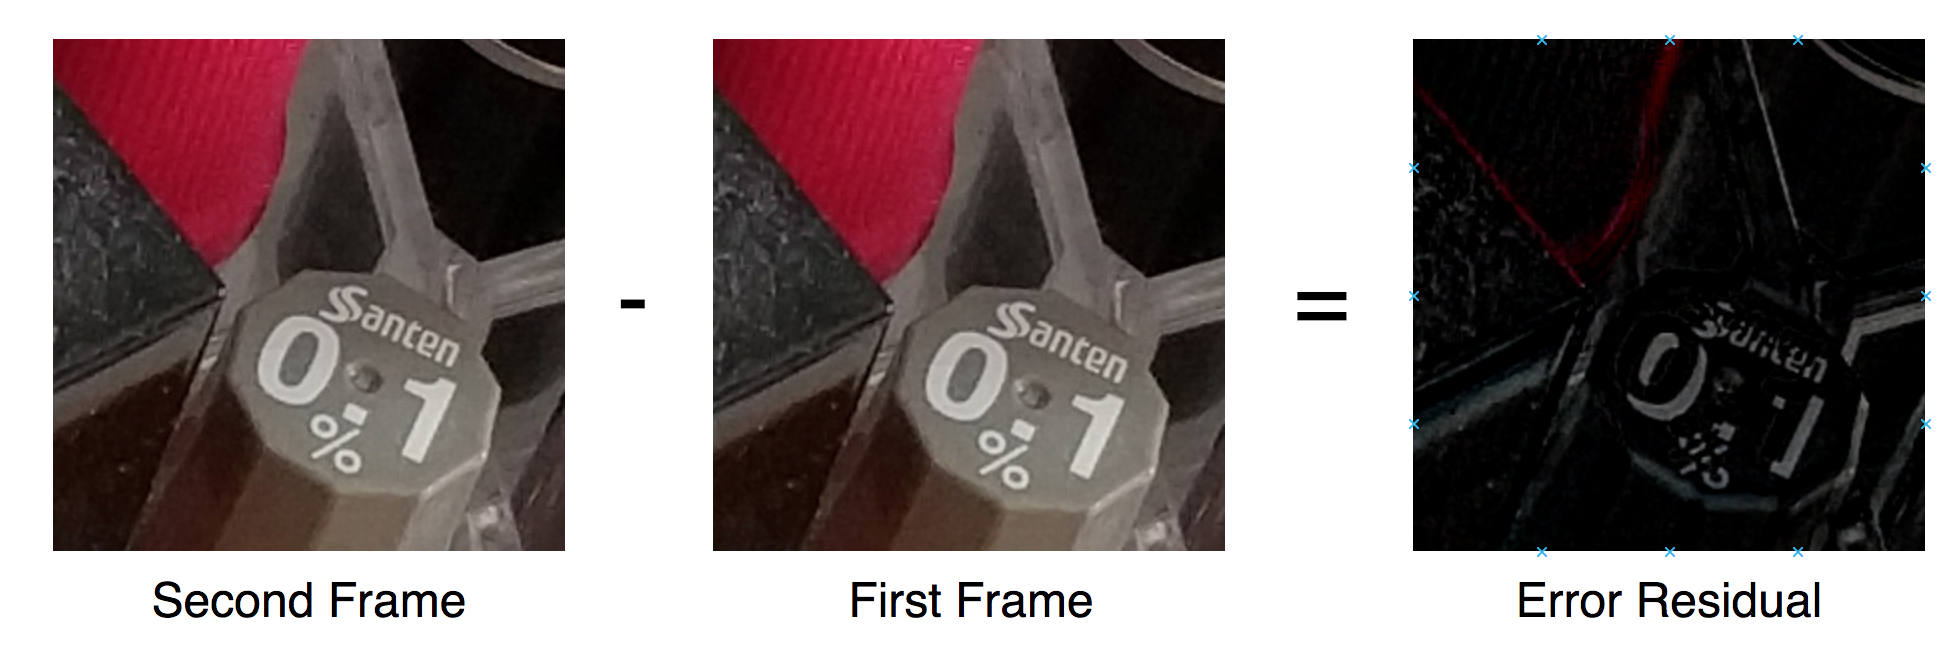
\includegraphics[width=0.9\linewidth]{Background/error_residual_vis.png}}
\caption{Visualization of a Video Prediction Error Residual}
\label{residualvis}
\end{figure}

MPEG-2 takes both of these concepts a step further. Both temporal and spatial redundancy are exploited in the frame prediction process. Successive video frames are first grouped together to minimize prediction error. The first frame in the group is encoded entirely using a JPEG-like process. This frame is called an intra-coded frame or I-frame. Following this I-frame is a sequence of predicted frames. Predicted frames come in two types. Regular predicted frames or P-frames derive their predictions from past frames. Bi-directional frames, or B-frames can mix predictions from both past and future frames. These groupings of frames are called groups of pictures (GOPs).

\begin{figure}[htbp]
\centerline{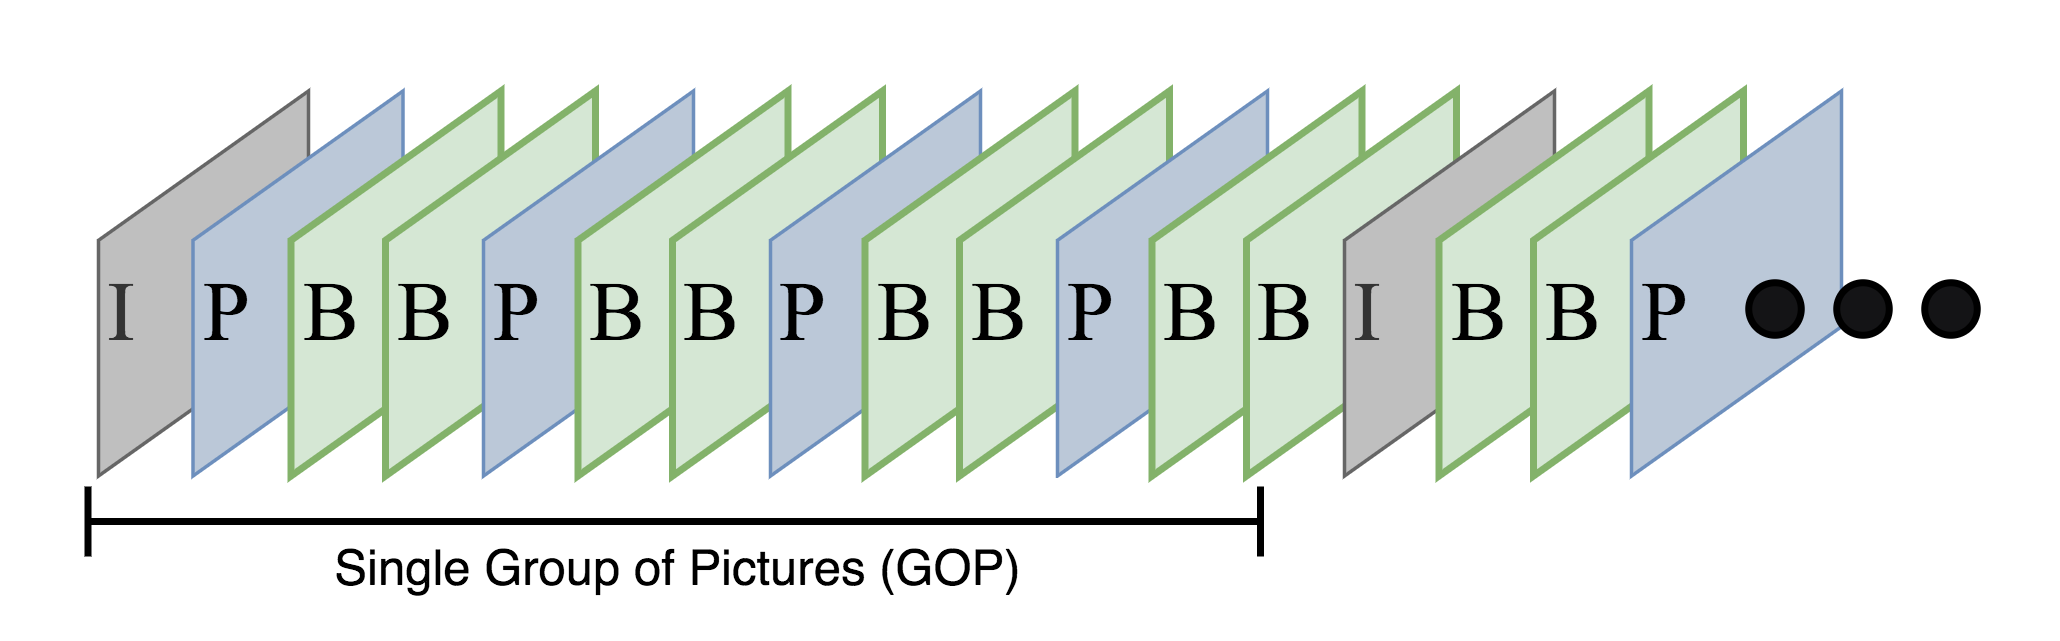
\includegraphics[width=0.9\linewidth]{Background/gop_example.png}}
\caption{Example of a GOP Sequence}
\label{exampleGOP}
\end{figure}

An example GOP sequence can be seen in Fig.~\ref{exampleGOP}. In most modern codecs, including MPEG-2, these GOP structures do not have to be fixed in size. The GOP length is determined by the distance between subsequent I-frames. Often, it is more efficient to make the GOP smaller during segments of high motion in a video. This is known as variable GOP encoding, versus fixed GOP encoding where the GOP sequence is always the same length.

Predictions can only be derived from I or P-frames, sometimes referred to as anchor frames. In MPEG-2, P-frames can only derive their predictions from a single previous anchor frame, while B-frames can derive their predictions from both a single previous and a single future anchor frame \cite{mpeg2}. To decrease the prediction error, predicted frames are partitioned into 16x16 pixel regions called macroblocks. These macroblocks are compared with blocks in the previous anchor frame and/or the next anchor frame in the case of B-frames. A fast search algorithm is performed to find a macroblock sized region with the smallest error when subtracted from the macroblock of interest.

The pixel displacement in both the x and y directions from the centroids of the macroblocks is stored in what is known as a motion vector. Then the error residual between the two macroblocks mapped by the motion vector is also stored. In this way, predicted frames are transmitted as a set of motion vectors and macroblock sized prediction error residuals. Decoding a predicted frame requires using the motion vectors to obtain the pixel values of the source macroblock for each macroblock in the frame. Then the error residual for each macroblock is added back, thus reproducing the original picture. The entire prediction error and motion vector generation process is known as motion compensation and estimation.

The H.264 specification contains many advancements in the motion compensation and estimation process \cite{h264} \cite{h264Overview}. Macroblocks no longer have to be 16x16 pixel blocks, and instead can be a variety of shapes including 8x16, 16x8, and 8x8. Single macroblocks can be encoded like an I-frame, instead of being predicted. These I-blocks are useful in scenes with high motion. Also, macroblocks can derive predictions from other portions of their frame. Intra-frame predictions are useful for large, mostly single colored regions like the sky. In this way, only one inter-frame motion vector has to be produced for an entire section of the image. It is also possible for the encoder to entirely skip a prediction for a given macroblock. Instead, the macroblock is directly copied from a previously decoded frame. These are known as skip macroblocks, or S-blocks.

The most notable improvement from H.264 over MPEG-2 is the ability for the encoder to have a substantially larger frame buffer. This allows for macroblocks in predicted frames to derive the motion vectors from across multiple different anchor frames. Effectively, a B-frame could be composed of macroblocks sourced from all anchor frames in the encoder's frame buffer. This substantially reduces the prediction error of any given macroblock. Fig.~\ref{multipred} shows an example of this. The first B-frame can source macroblocks from any I and P-frame within the GOP that is resident in the encoder's frame buffer.

\begin{figure}[htbp]
\centerline{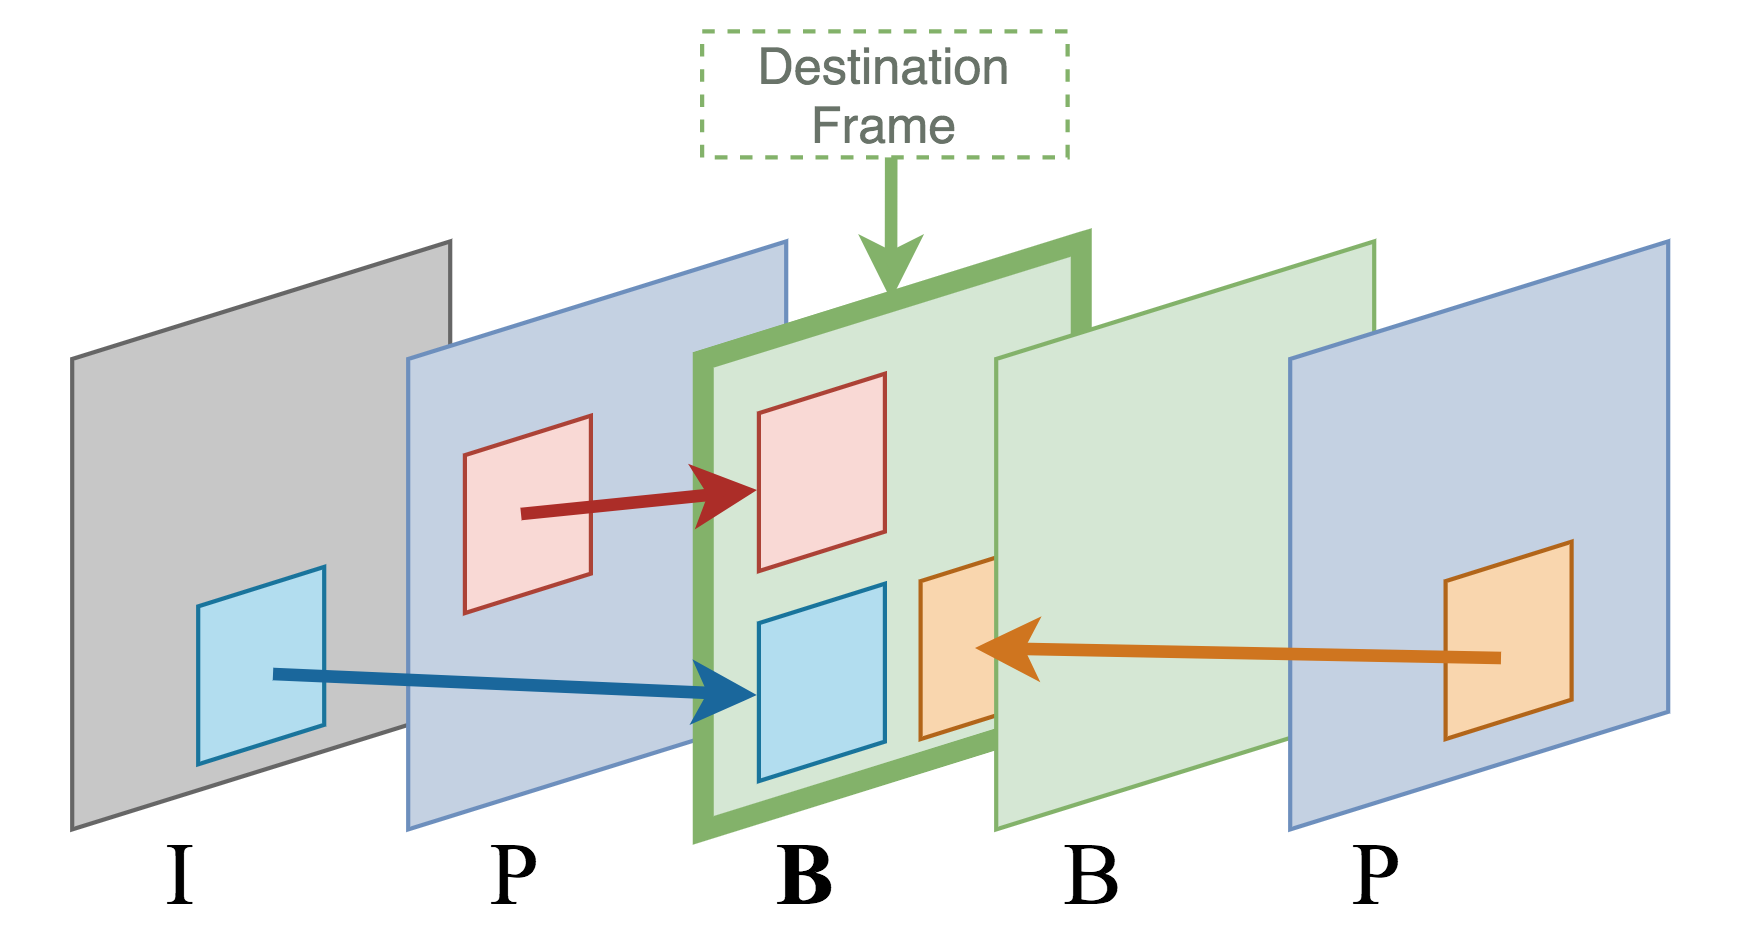
\includegraphics[width=0.9\linewidth]{Background/multi_frame_pred.png}}
\caption{Visualization of Using Multiple Anchor Frames for Prediction in H.264}
\label{multipred}
\end{figure}

\section{Frame Deletion Detection}

Detecting the tampering of a video uses similar general techniques that were originally used for detecting tampering in images. In most cases, a statistical fingerprint is extracted from the media source which contains information about the specific method of tampering an investigator wishes to detect. Frame deletion detection in video was originally found to create two distinct fingerprints in the underlying video \cite{wang}. 

One of these fingerprints is spatial in nature. When a video has had frames removed from it using video editing software, the video must first be decoded. One can simply store the decoded video without recompression, but then they would run into storage limitations as shown previously. Thus, it is common to recompress a video after removing frames. In this manner, detecting frame deletion in video is related to detecting double compression of video. Due to the JPEG-like process of encoding I-frames, Wang and Farid show that a similar fingerprint to the one used to detect double JPEG compression \cite{doubleJPEG} \cite{doubleJPEG2} is found in the I-frames of doubly compressed MPEG video. Note that this fingerprint occurs even if no frames are removed from the video \cite{wang}. Thus, more information is needed to determine whether or not a video has had frames removed from it.

The temporal fingerprint observed by Wang and Farid can make this distinction \cite{wang}. The temporal fingerprint occurs due to the structure of the motion compensation and estimation process in MPEG-2 encoding. In each GOP, the statically compressed I-frame is inserted to prevent excessive buildup of motion estimation errors. The first P-frame in a GOP is thus directly encoded with respect to the I-frame. As each subsequent P-frame in the GOP is encoded based on the previous P-frame, it can be said the these P-frames are indirectly encoded with respect to the initial I-frame. As well, the content of each P-frame is found to be correlated with the I-frame. Wang and Farid explain this phenomenon as the result of the JPEG-like compression process of the I-frame \cite{wang}. The compression artifacts propagate through the P-frames resulting in each P-frame being correlated to its previous anchor frame. In addition, the correlation between P-frames in different GOPs is reduced compared to the correlation within a single GOP.

\begin{figure}[htbp]
\centerline{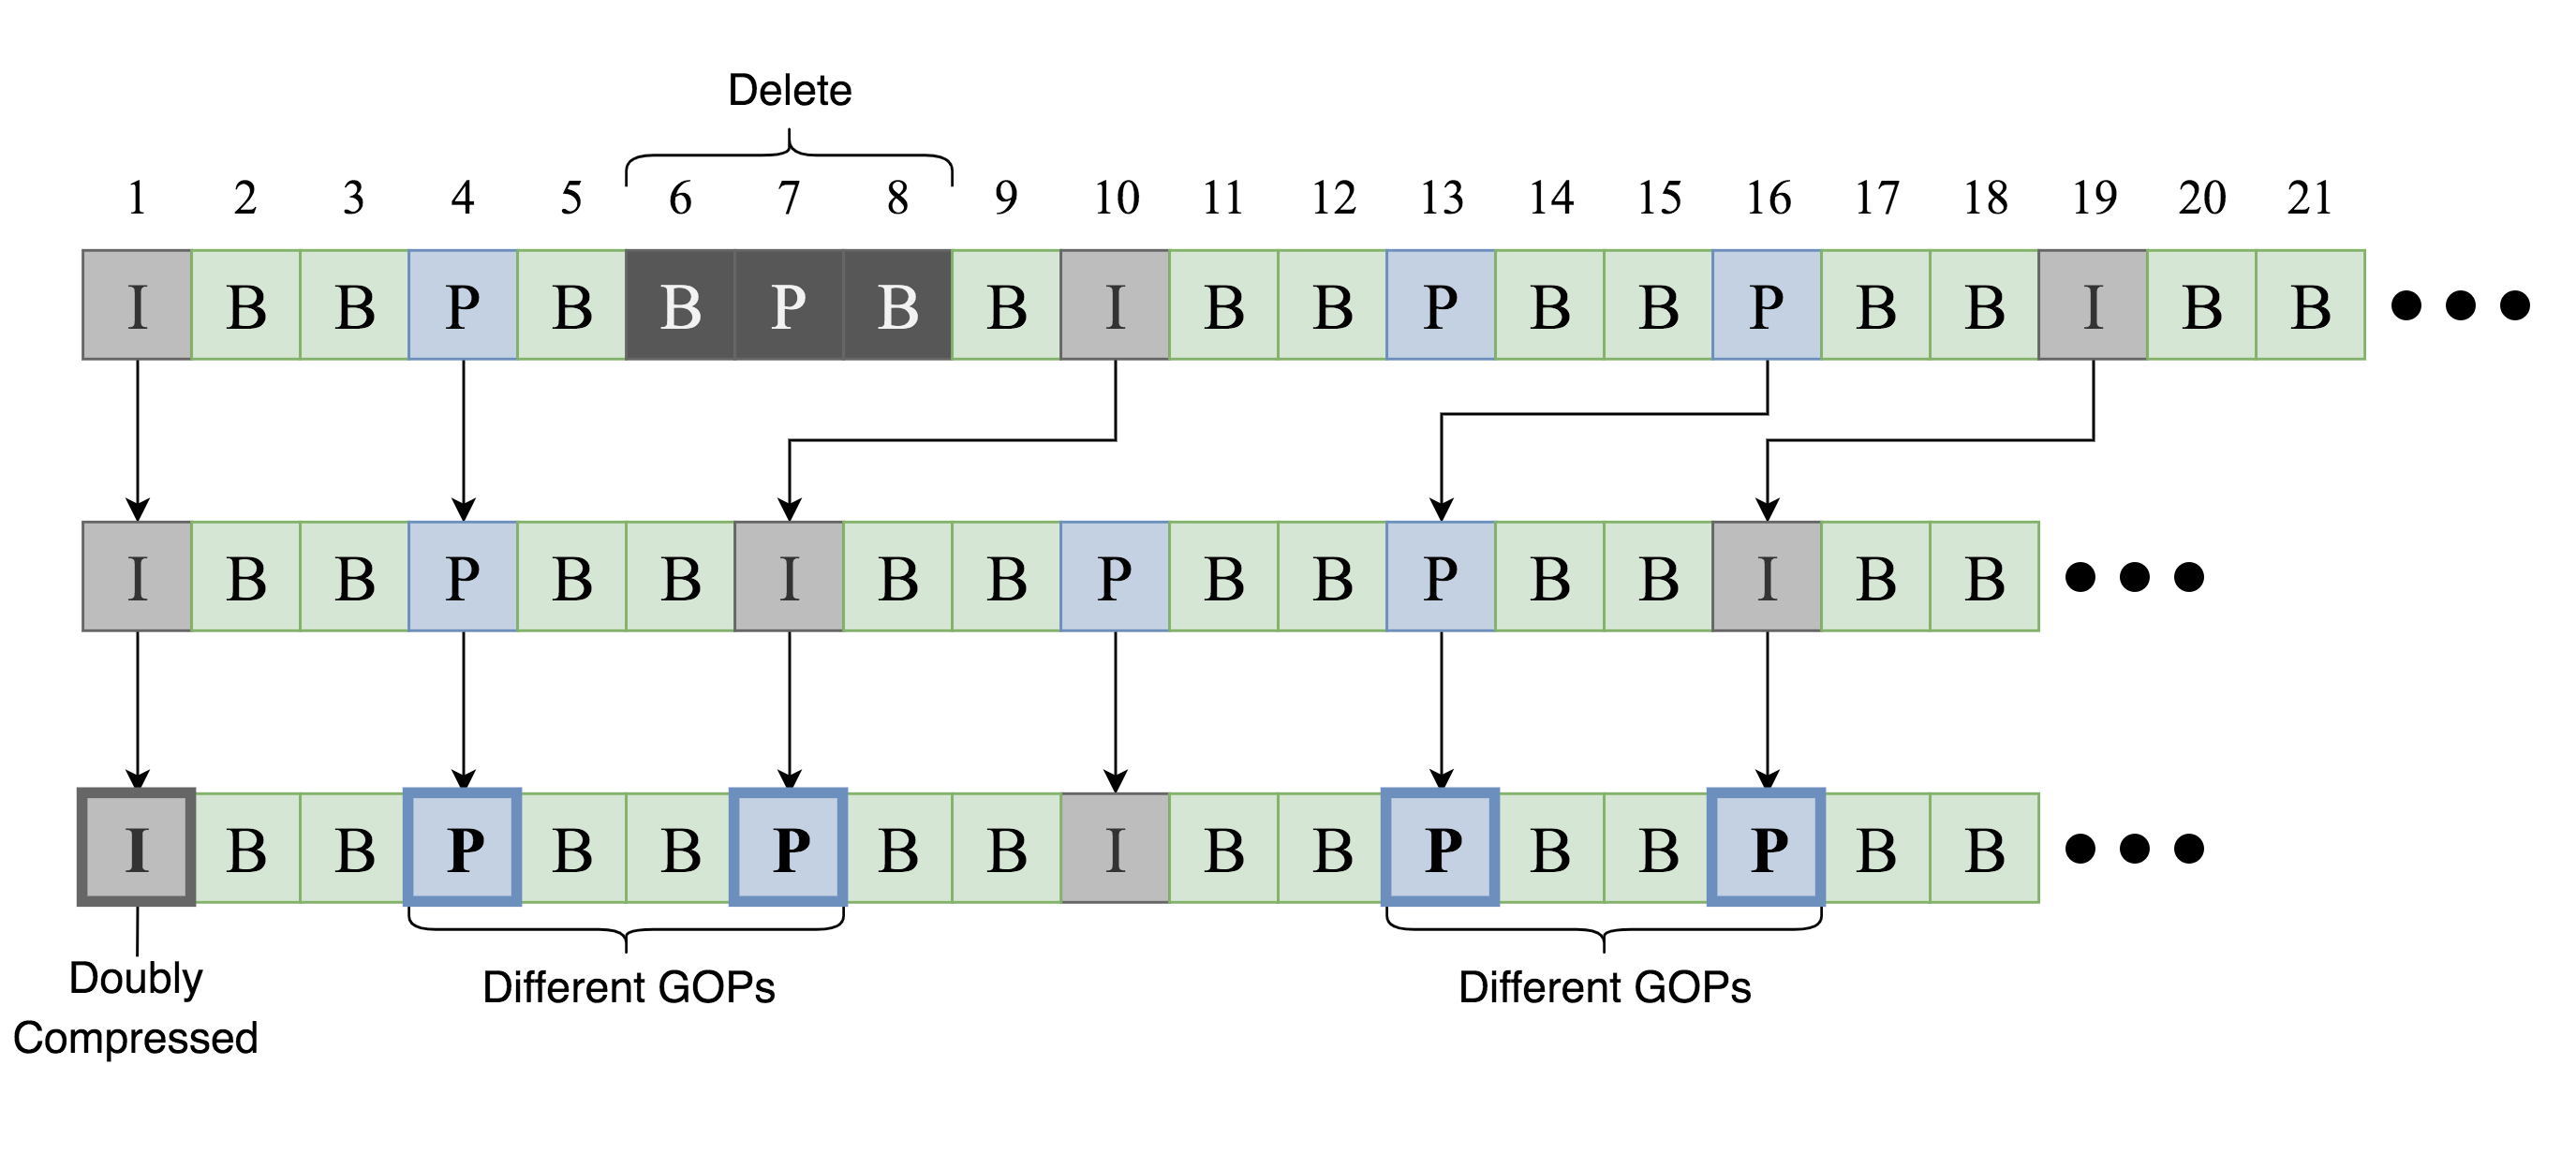
\includegraphics[width=0.9\linewidth]{Background/frame_deletion.png}}
\caption[Visualization of the Effects of Frame Deletion on a Sample MPEG-2 Encoded Video.]{Visualization of the effects of frame deletion on a sample MPEG-2 encoded video. The top row shows the original encoded sequence, while the bottom rows show the effects of deleting the three highlighted frames.}
\label{framedeletion}
\end{figure}

When frames are removed from a video, the new sequence of frames has GOPs that contain frames from across multiple GOPs in the original unaltered video. As a result, some frames can change type, and predicted frames can derive their predictions from frames originally in another GOP. This effect can be seen in Fig.~\ref{framedeletion}. Frames 6-8 were removed from the original video sequence. Note that frame 13 has become an I-frame when it was originally a P-frame, and frames 10 and 19 have become P-frames when they were originally I-frames. When frames derive their predictions across GOP boundaries, the correlation between the frames is lower, and thus there is an increase in prediction error. Wang and Farid show that for fixed GOP videos, this increase is periodic with respect to the length of a GOP.

As such, Wang and Farid proposed observing the average inter-frame prediction error for each P-frame in a given video. If there are periodic spikes in this P-frame prediction error sequence, then the video has had frames removed from it. While Wang and Farid showed that this fingerprint exists, they did not formulate a detection algorithm for this fingerprint, nor did they test the effects of frame deletion on variable GOP video. They relied on visual inspection of the Discrete Fourier Transform (DFT) of the P-frame prediction error sequence for detecting frame deletion.

Further work was done by Stamm et al. \cite{stamm} \cite{C} on using the temporal fingerprint proposed by Wang and Farid to detect frame deletion in MPEG-2 video. Stamm et al. proposed an initial model for the fingerprint itself, and how to separate an estimate of the fingerprint from a given P-frame prediction error sequence. They then formulated two decision rules based on the estimated fingerprint signal. One was for fixed GOP video, and the other was for variable GOP video. The variable GOP decision rule was found to also work for fixed GOP video as well, since it was based on the total energy in the estimated fingerprint signal.

This work still had limitations. First, it is not clear whether this detection method is robust to advancements in video encoding, particularly the ability for H.264 to derive motion vectors across multiple anchor frames. As well, both Stamm et al. and Wang and Farid were limited in the type of data they were able to generate for their experiments. They both used video with carefully controlled processing histories that are not necessarily representative of video that can be found in real world scenarios.

\subsection{Frame Deletion Detection on H.264}

Work on frame deletion detection in more modern video codecs, such as H.264 or MPEG-4 so far has been limited. Techniques have been proposed based on Wang and Farid and Stamm et al.'s original solutions for MPEG-2. However, they only cover video without B-Frames and the scenario where the altered video undergoes recompression with a different GOP size after frames have been removed \cite{Liu}. Another technique based on detecting mismatches in image sensor based traces within a video \cite{Mandelli} is able to detect video splicing, where content is stitched together from multiple camera sources. However, this technique may not work on video take only from one camera, as well as video that has undergone motion stabilization, a post-processing technique found in many smartphone cameras.

Of particular note is a technique proposed V\'azquez-Pad\'in et al. \cite{Vazquez} They found that when H.264 video is reencoded, particularly when GOP sizes do not match between encodings, the number of I-blocks and S-blocks vary from expected values when P-frames are encoded as I-frames and vice-versa. V\'azquez-Pad\'in et al. showed that it is possible to use this mismatch to determine whether an H.264 video has been recompressed \cite{Vazquez}. This technique was expanded upon by Gironi et al. \cite{barni}. As videos that have undergone frame deletion will naturally have frames change type upon reencoding, the same mismatch in the number of expected I and S-blocks appears in videos with frame deletion as well. Gironi et al. reformulated the proposed fingerprint by V\'azquez-Pad\'in et al. to work in this context. However, the method proposed by Gironi et al. is unable to work on video that has a variable GOP size.

\section{Autoregressive Models}

In our proposed frame deletion detection technique we use a statistical forecasting model called an autoregressive (AR) model. Here we describe how it works. An AR model is a statistical model of a stochastic process. The model seeks to predict future values of the process based on past observations. They are used for forecasting when there is some correlation between the values within the process. The future values are modeled as a linear combination of past observations (called lag variables) and white noise. You only use data from the same process to model the future values, thus the name "autoregressive". Effectively an AR model is a linear regression of the past data in a stochastic process where the target value is a future value of the process.

The model order of an AR model depends on the number of lag variables used in calculating the future values. Thus for a $M^{th}$ order AR model, the current value of the time series $u(n)$ is defined as

\begin{equation}
u(n) = \sum_{k = 1}^{M} w^{*}_{k} u(n-k) + v
\end{equation}

where $w^{*}_{1}, \dots, w^{*}_{M}$ are the AR model parameters $v$ is white noise. The variance of the white noise component determines the degree to which the model is able to fit the stochastic process. AR models are solved using the Yule-Walker equations as found in \cite{ARmodels}. In this work, we use the AR model parameters for a given video to characterize the properties of the frame deletion fingerprint. In doing so, we are able to account for the natural variance between videos in our decision-making process.

\section{Support Vector Machines}

In order to make a decision as to whether a video has had frames removed from it, we use a Support Vector Machine (SVM) classifier. SVMs are a widely popular machine learning technique for classification \cite{svm}. The goal of an SVM is to learn an optimal separating hyperplane between classes of data by maximizing the margin between the data points in each class that are closest to data points in the other classes. These closest points are known as support vectors. The support vector machine learns a discriminate function based on these support vectors. The SVM does not make a probabilistic model of the data to determine classification. However, there are techniques \cite{plattscaling} to scale the data in such a fashion that the SVM can return an estimate of the probability that a data point is from a particular class. Fig.~\ref{svmvis} shows an example of creating a binary decision function  using an SVM.

\begin{figure}[htbp]
\centerline{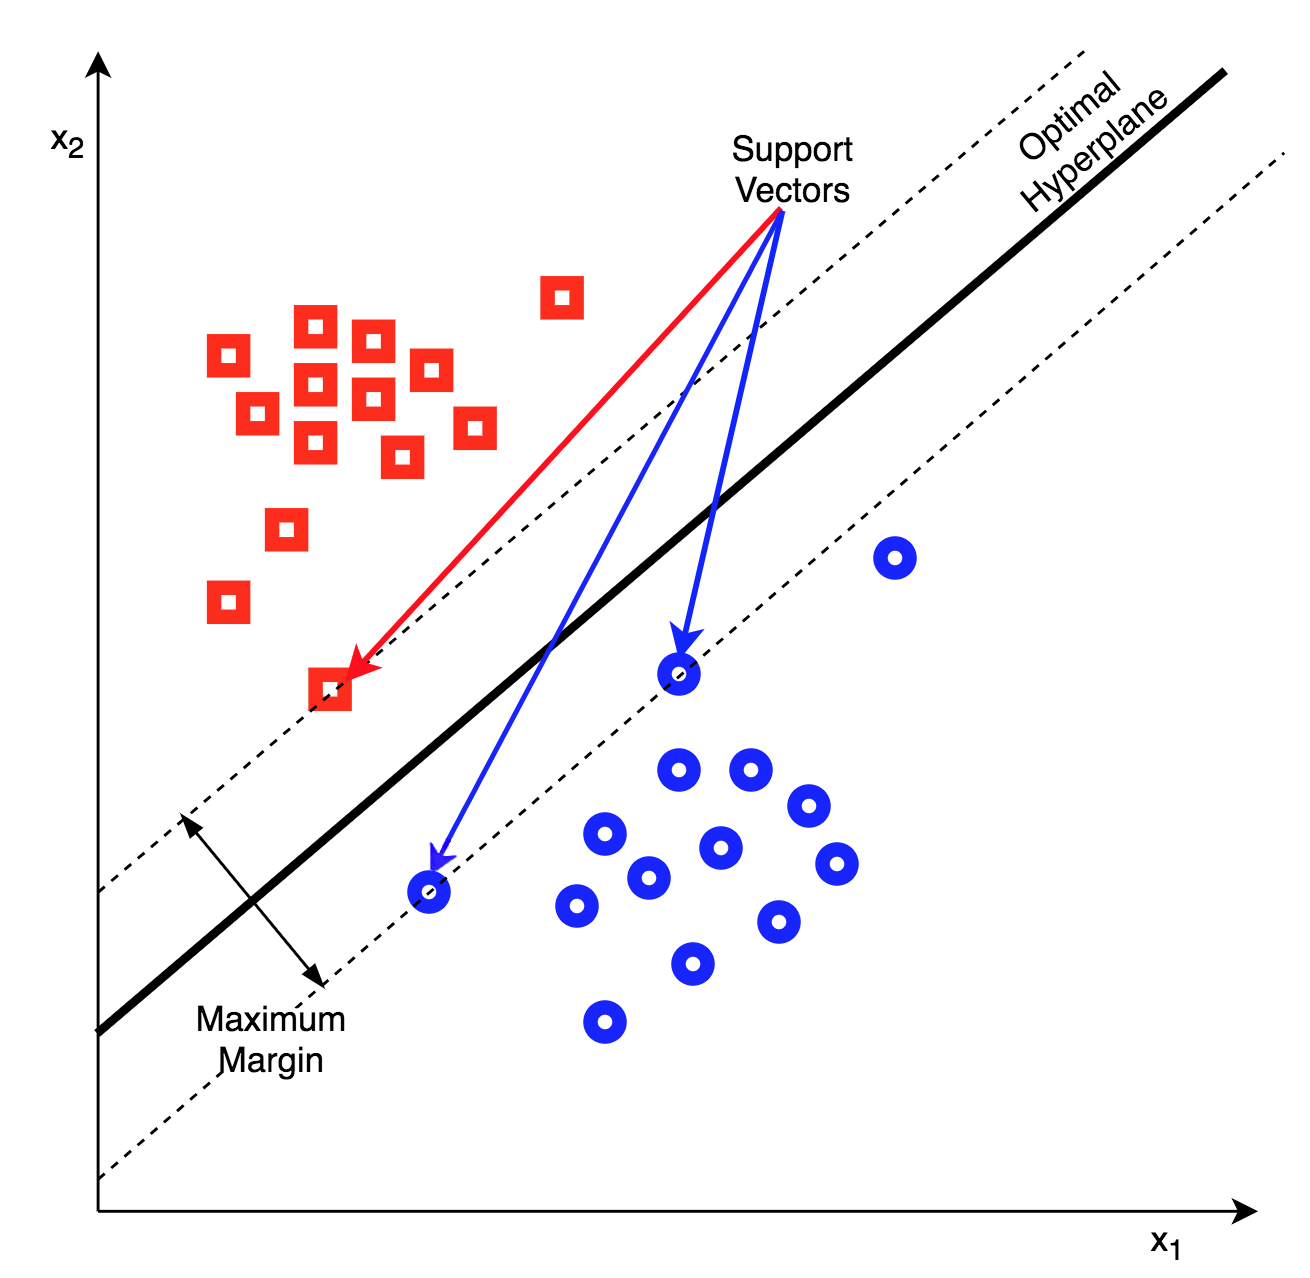
\includegraphics[width=0.7\linewidth]{Background/svm_vis.png}}
\caption{Visualization of the Optimal Hyperplane Learned by an SVM }
\label{svmvis}
\end{figure}

An SVM can use a kernel function to map the input data into higher dimensional space. Depending on the mapping, it is possible to further separate the distance between classes. This means that an SVM can learn nonlinear decision surfaces, given the right kernel. One of the most popular kernels to use is the radial basis kernel. The radial basis kernel projects the data onto a Taylor series expansion of a gaussian distribution.

% This file is for the problem formulation section of the Master's Thesis.
% This file will not compile on it's own. Will need to include it into a main file
% That uses the drexel thesis template.
\chapter{Problem Formulation}

Detecting frame deletion in a video requires detecting the structural changes in a video due to the deletion process. In particular, Wang and Farid's work on temporal traces for detecting frame deletion shows that for MPEG-2 video, the P-frame prediction error can be formulated into a sequence. This sequence can then be monitored to detect frame deletion. Both Wang and Farid, and Stamm et al. use a system like in Fig.~\ref{System} to detect frame deletion. The prediction error sequence $e(n)$ is extracted from the decoded video file and processed to produce detection features. Wang and Farid's work did not propose features for automatic detection, and instead relied on visual inspection of the DFT of the prediction error sequence \cite{wang} \cite{stamm}.

\begin{figure}[htbp]
\centerline{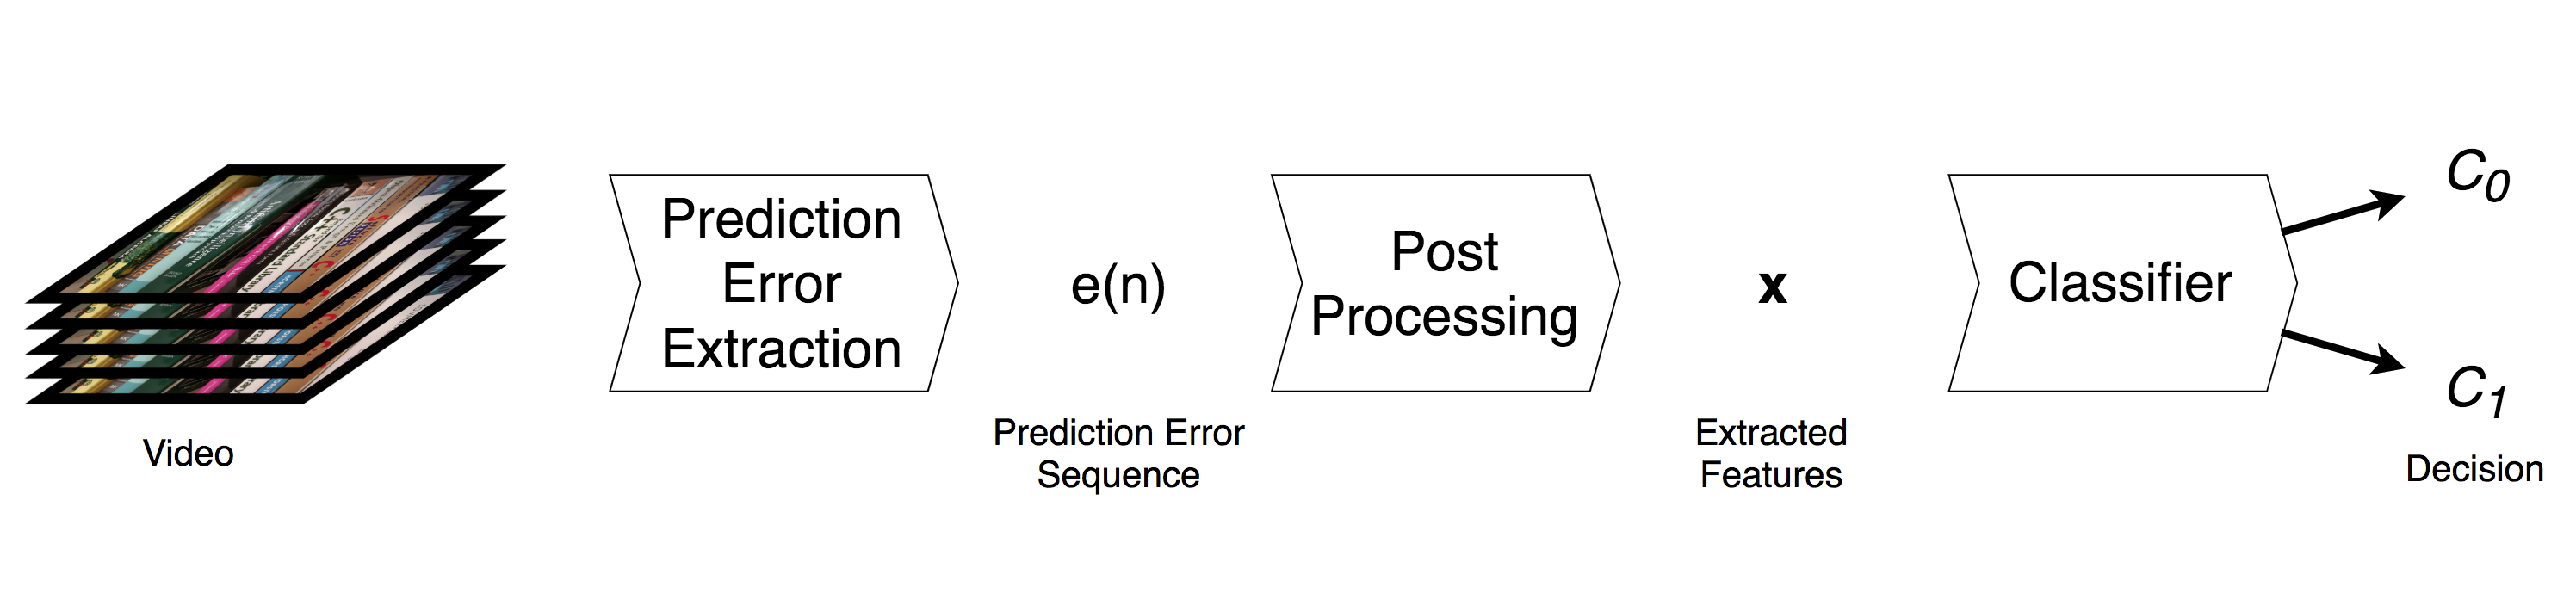
\includegraphics[width=0.9\linewidth]{ProblemFormulation/frame_deletion_detection_system.png}}
\caption{Generalized Approach to Frame Deletion Detection}
\label{System}
\end{figure}

This broad approach can also be applied to work with H.264 encoded video as well. While video encoding has advanced significantly, the fundamental structures of a compressed digital video have remained unchanged. Regardless of codec, the hallmark of video compression is the motion compensation and estimation process. Video frames are organized into GOPs that begin with an I-frame, and have varying structures of P and B-frames. In H.264, GOP structures are more dynamic due to the ability to derive motion-vector predictions from across multiple anchor frames. To remain robust to these advances in video compression, the prediction error extraction and post processing steps must be altered or augmented.

This work is concerned particularly with the detection of frame deletion in H.264 and similar modern video codecs. Frame addition has also been observed to introduce similar traces in the P-frame prediction error sequence as frame deletion. Our proposed system can be applied to detecting frame addition and for simplicity we will not discuss the detection of frame addition for the remainder of this thesis. We have made the following assumptions regarding our proposed system. First, we assume that all altered video has undergone re-compression. In fact, since most consumer video recording devices do not have the storage capability or processing power to record high-definition raw video, it is assumed that all video sources have been compressed by either MPEG-4 or H.264, and that all frame deleted video will be re-compressed using H.264 or a similar codec, where the reencoding is set to match the GOP structure of the source video. 

In addition, it is assumed that all videos that are passed to the detector are of sufficient length to make a classification. Without multiple full GOPs, the presence of a deletion fingerprint is negligible. Lastly, we make the assumption that if indeed frames have been removed from a video, they have not been removed from the end of the video. The detection features are dependent on differences between the structure of the prediction error sequences in natural videos versus videos with frame deletion. When frames are removed from the end of the video sequence, this difference is not observable. 

A user of our proposed system will not need physical access to a specific device to analyze a video captured by the device. The system should accept videos of an arbitrary length, and will not require metadata unrelated to video playback to be intact. It will work with videos of any resolution, frame rate, or GOP structure. Also, as our approach will be data driven, it is imperative that a user have access to a sufficient database of videos with known labels.

\section{Video Frame Deletion Detection}

Detecting frame deletion is a binary classification problem. Given a Video $V$, there are two possible classes:

\begin{equation}
\begin{aligned}
  C_{0} &: \text{The video is genuine, and has not had frames removed from it.} \\
  C_{1} &: \text{The video is altered, and has had frames removed from it.}
\end{aligned}
\end{equation}

Note that in this case, \emph{genuine} refers to the fact that the video has not undergone any additional post processing after its original capture. We will simply be considering the limited scenario whereby video has either come directly from the camera that captured it, or frames have been removed from the video and it has been recompressed. Any mention of a genuine video for the rest of this thesis refers to a video that has not been modified since it's original capture.

In general, it is difficult to classify whether or not a video has had frames removed based on the entirety of a video directly. Thus, the problem must be reworked. As shown above, a feature extraction system will be used to produce the P-frame prediction error sequence $e(n)$, and a feature vector $\bm{x}$. The feature vector ideally contains information about the prediction error sequence that can perfectly separate the two classes. As such, the classification problem is as follows. Given a feature vector $\bm{x}'$, it belongs to one of two classes:

\begin{equation}
\begin{aligned}
  C_{0} &: \bm{x}' \text{resulted from a genuine video that has not had frames removed from it.} \\
  C_{1} &: \bm{x}' \text{resulted from an altered video which has had frames removed from it.}
\end{aligned}
\end{equation}

In the following chapter, we will propose both a new method for extracting $e(n)$, and additional augmentations to $\bm{x}$ that allow for improved separation of data and increased robustness of the overall system.

\chapter{Proposed Approach}

\section{Prediction Error Sequence Extraction}

In previous work on frame deletion detection in MPEG-2, the prediction error sequence was extracted directly from the video decoder using the DCT coefficients of the prediction error residuals located in the compressed video file. The prediction error was averaged over all macroblocks in a frame. This prediction error was then stored as a sequence. Due to the nature of the correlation between P-frame prediction errors across a single GOP, any prediction made across GOP boundaries would result in increased prediction error. Wang and Farid showed that for fixed GOP video, the increase in average prediction error is periodic with respect to the number of frames deleted from the video. Stamm's work expands the idea of the prediction error trace by introducing the formulation of a fingerprint signal defined like so:

%TODO Put equations in for the definition of the the fingerprint signal s_hat

This fingerprint signal can be used to build a detector for both variable and fixed GOP videos. Despite this advance in detection, the underlying method for extracting the prediction error sequence is the same.

In MPEG-2, a P-frame is encoded by searching the previous anchor frame for the macroblock which incurs the least error. This means that the average prediction error for a single P-frame is only asssociated with the previous I or P-frame. H.264 expands the capabilities of its motion compensation and estimation system by allowing prediction from multiple previous frames (and subsequent frames in the case of B-frames). If the prediction error trace is extracted via the codec for H.264, the average prediction error associated with one frame is comprised of a linear combination of the average prediction error associated with motion vectors that map to the different anchor frames used in the motion estimation and compensation process. Thus, cross GOP predictions are smoothed out in such a way that it makes the fingerprint energy detector in Stamm's paper perform inadequately.

%TODO Put figure from stamm's paper showing the detection ROC
%TODO Show the detection ROC for the original methodology on H.264

As shown in Fig. ~\ref{•} the probability of detection using the methodology from MPEG-2 videos does not translate to H.264. Instead, we propose the following methodology for extracting the prediction error sequence in H.264.

\subsection{Proposed Prediction Error Sequence Extractor for H.264}

The goal of the proposed extraction algorithm is to maximize the probability that should frame deletion exist, a given measurement of the prediction error comes from a cross-GOP prediction. To this end, instead of directly measuring the prediction error from the DCT coefficients from the decoder, we decode the frame of interest and store the motion vectors associated with said frame. For each macroblock in the current frame, we use its associated motion vector to find the x and y coordinates defining the source macroblock which provides the least error mapping from a previous anchor frame. Then for a previous anchor frame, we subtract the pixels in the source macroblock from the destination macroblock in the current frame. This leaves us with a prediction error residual associated with the macroblock. We then calculate the average absolute value of this residual.

%TODO Insert Figure Showing Identification of Macroblocks in multiple previous frames

We repeat this process for each of D previous anchor frames. Then we store these prediction error values in a matrix $M$, where each row of the matrix corresponds to the errors associated with a single motion vector, and the columns are the errors associated with each of the previous anchor frames.

After obtaining the $M$ matrix for the current frame, we create the matrix $\tilde{M}$ defined like so:

\begin{equation}
  \tilde{M}_{i, j} = \mathds{1} \left(j == \argmin_{l} \left( M_{i, l} \right) \right) * M_{i, j}
\end{equation}

Thus $\tilde{M}$ is a copy of $M$ where the non-zero entries in each row correspond to the minimum average error associated with the macroblock and all other elements are zero. Effectively, the column index of the non-zero entry is an estimation of which previous frame the motion vector associated with the macroblock maps to in the decoding process.

Further processing is done on $\tilde{M}$ to output only a single prediction error value. First, $\tilde{M}$ is reduced into a vector $P$, such that:

\begin{equation}
  P_{j} = \frac{1}{N_{j}} \sum_{i}{\tilde{M}_{i,j}}
\end{equation}

Where $N_{j}$ is the number of non-zero elements in the $j^th$ column of $\tilde{M}$. Then, the reported prediction error $e$ is set as the maximum value of $P$. This entire process is repeated for every P frame in the video. This method of error extraction estimates which previous anchor frame contributes the maximum error per macroblock to the overall prediction error residual obtained by the codec for a given P frame. Since prediction across GOP boundaries results in spikes in the prediction error, the anchor frame that contributes the most error is most likely to be from a different original GOP. In this manner, we obtain a trace that is resilient to advances made in the motion compensation and estimation process in modern codecs as well as robust to variable frame rates and dynamic GOP structures.

\section{Proposed Detection Algorithm}

In addition to the new methods for prediction error extraction, we propose an expanded detection algorithm to better capture the statistical differences between videos. In fact, depending on scene content, video capture settings, and the amount of motion captured in a single recording, the prediction error sequence and fingerprint signal exhibit different structural behavior. This is true even for videos captured from a single camera model. Figure ~\ref{} shows this clearly. The two videos were captured from a *insert phone here* using the high quality 1080p capture mode. Both videos were shot using similar scene content, but the amount of motion in the video is different. The top row shows the different prediction error sequences, while the bottom row shows the fingerprint signals.

%TODO Insert figure comparing the two videos' fingerprint signals and prediction error seqs

Thus there is a need to construct a parametric model of the fingerprint signal and the prediction error sequence to capture these statistical variations. We propose constructing an autoregressive (AR) model of both the fingerprint signal and the prediction error sequence. Over the time period of one GOP it can be said that the signals are mostly stationary. The parameters of the AR models are added to a feature vector along with the fingerprint energy described above. In order to capture the degree to which this is true, the error variance of each AR model is also included. In addition, some basic statistical features are included to scale the overall decision surface. We propose including the mean and variance of both the prediction error sequence and fingerprint signal to the feature vector as well.

Note that after creating a feature vector for each video, the feature vector is quite large. It is inadvisable to create a probabilistic model of the feature vector for classification. Instead, we propose using a discriminative function to map an incoming feature vector directly to the set of natural videos or the set of videos altered by frame deletion. As such, we propose using a Support Vector Machine (SVM) classifier with a Radial Basis Kernel function for classification.
\chapter{Experimental Results}

We conducted a series of experiments to evaluate both the performance of our proposed prediction error extraction algorithm and new detection features. In order to create a suitable dataset for our experiments, we gathered a set of at least 250 five second long video clips from a variety of camera models. As the video processing pipeline is different between camera models, we aimed to include a diverse set of GOP structures. To create our frame deleted videos, we then removed 15 frames from the beginning of each video in our dataset. The reencoding was handled using the x264 library, and we matched the original GOP structure of each video for the frame deleted copy. We then filtered out all videos with less than 60 P-frames, as having fewer than 60 P-frames is not sufficient for making a reasonable classification of a video sequence. The resulting dataset can be found in Table ~\ref{datasetComp}.

\begin{table}[htbp]
  \begin{adjustbox}{width=0.9\linewidth, center}
  \begin{tabu}{ l | l | c | c | c | c }
    \hline
    \rowfont{\bfseries} Camera Model & GOP Type & GOP N & GOP M & Genuine Videos & Frame Deleted Videos \\ \hline	
    ASUS ZenFone 3 Laser & Fixed & 30 & 1 & 257 & 257 \\
    Apple iPhone 8 plus & Variable & 30 & 2 & 248 & 245 \\
    Google Pixel 1 & Variable & 29 & 2 & 776 & 777 \\
    Google Pixel 2 & Variable & 29 & 2 & 212 & 212 \\
    Kodak Ektra & Fixed & 30 & 1 & 503 & 502 \\
    Nokia 6.1 & Fixed & 30 & 1 & 501 & 500 \\
    Samsung Galaxy S7 & Fixed & 30 & 1 & 231 & 231 \\ \hline
    \textbf{Total Count} &  &  &  & \textbf{2728} & \textbf{2724} \\ \hline
  \end{tabu}
  \end{adjustbox}
  \caption{Composition of Frame Deletion Dataset}
  \label{datasetComp}
\end{table}

Note that GOP N is the maximum distance between I-frames in a video, which is the GOP length. GOP M is the maximum distance between P-frames in a video, thus a video with an M value of 1 has no B-frames at all. Note that some deleted videos had just enough frames removed to put them below the 60 P-frame threshold. Thus, there is a slight imbalance between the total number of videos present in each class. As well, data gathered from camera models with more than 275 videos was captured using multiple individual devices. The videos from the Google Pixel 1 contain footage captured on three devices, while the Kodak Ektra and Nokia 6.1 contain video from two devices.

\section{Single Camera Model}

To gauge relative performance of our proposed detection methods, we first tested on a single camera model. We chose to use videos from the ASUS ZenFone 3 Laser. When testing for the effects of our proposed prediction error extraction method, we used the decision metric proposed by Stamm et al. for MPEG-2 video, as described in Equation ~\ref{origdecision}. We varied the decision threshold used in each detector over a range of possible values. The probabilities of detection ($P_{D}$) and false alarm ($P_{FA}$) were measured for each value of the threshold. We then calculated the Receiver Operator Characteristic (ROC) curves for both prediction error extraction methodologies.

\begin{figure}[htbp]
\centerline{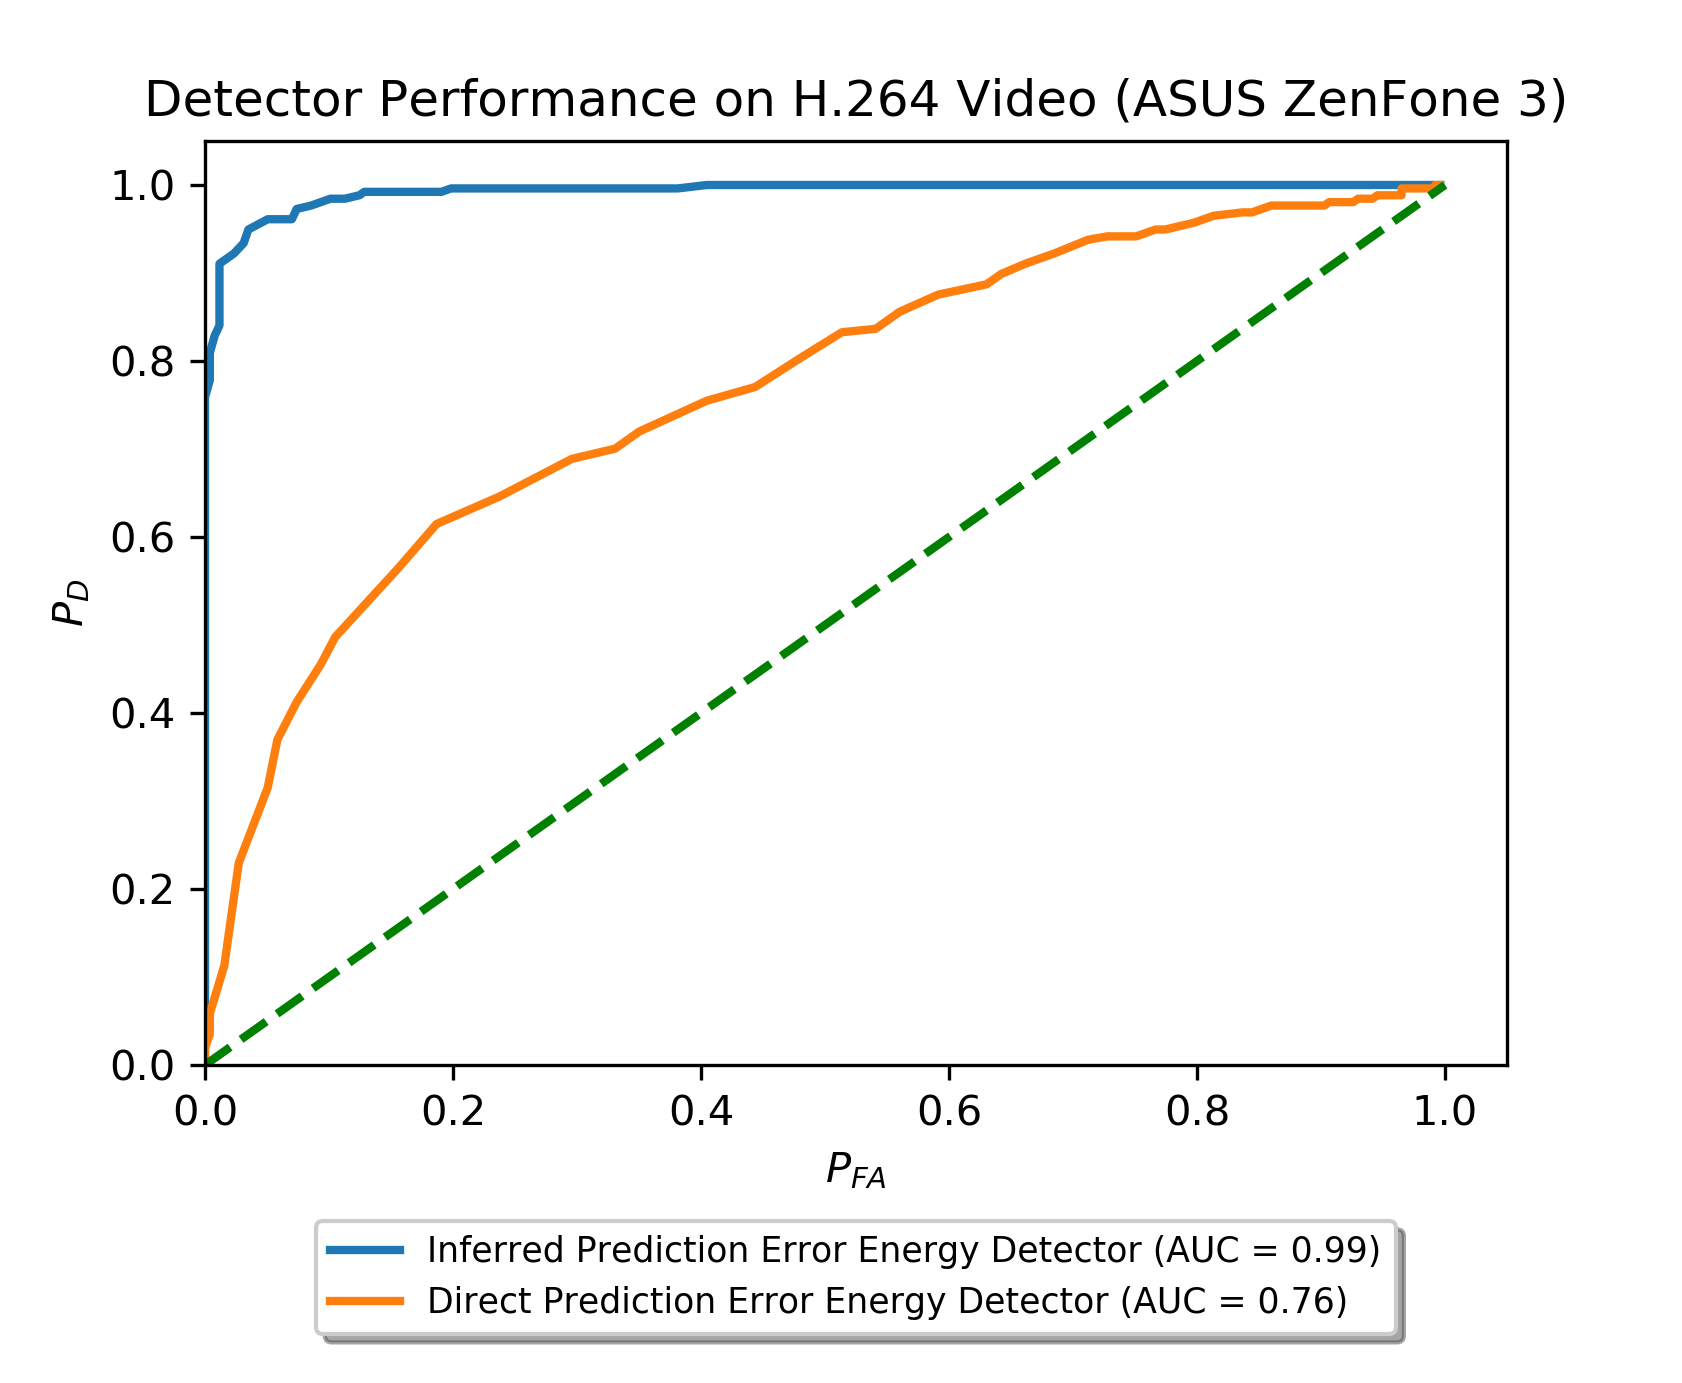
\includegraphics[width=0.7\linewidth]{ExperimentalResults/new_perror_extract_roc_asus.png}}
\caption{ROC Curves for Fingerprint Energy Detector Obtained by Using Different Prediction Error Extraction Methods}
\label{perrorExtractASUS}
\end{figure} 

As shown in Fig. ~\ref{perrorExtractASUS}, extracting the prediction error sequence directly from the codec (direct prediction error) results in poor detector performance. The detector build from the direct prediction error sequence is only able to reach 60\% detection rates at 20\% false alarm rates. Compare to our proposed prediction error extraction methodology (inferred prediction error). For the ASUS ZenFone3, we achieve over 90\% detection rates at less than 10\% false alarm rates. These results indicate that indeed our new inferred prediction error extraction methodology is able to yield separation between the two classes of data where the original direct prediction error extraction methodology does not, particularly at low false alarm rates. There is a delta upwards of 70\% in the probability of detection for a given false alarm rate.

Next, we examined the effects of using our proposed feature vector and an SVM on classification accuracy. We set the AR model orders for both the prediction error sequence and the fingerprint signal to 31. This is because of the periodic nature of the fingerprint on fixed GOP video. We want to predict when the signal will spike based on the previous GOP. We used the SVM with a radial basis function as the kernel and set the hyper-parameters of the SVM and the radial basis kernel to their defaults. To train the SVM, we partitioned our data into training and testing sets. The testing set was sized to be a quarter of the total dataset. Thus, there were 128 videos used for testing and 386 videos used for training. We set the SVM to use Platt scaling to return a probability instead of a class label \cite{plattscaling}. By doing so, we were able to vary the detection threshold and construct an ROC curve from the testing set for comparison with the fingerprint energy detector. The results can be seen in Fig. ~\ref{svmrocASUS}.

\begin{figure}[htbp]
\centerline{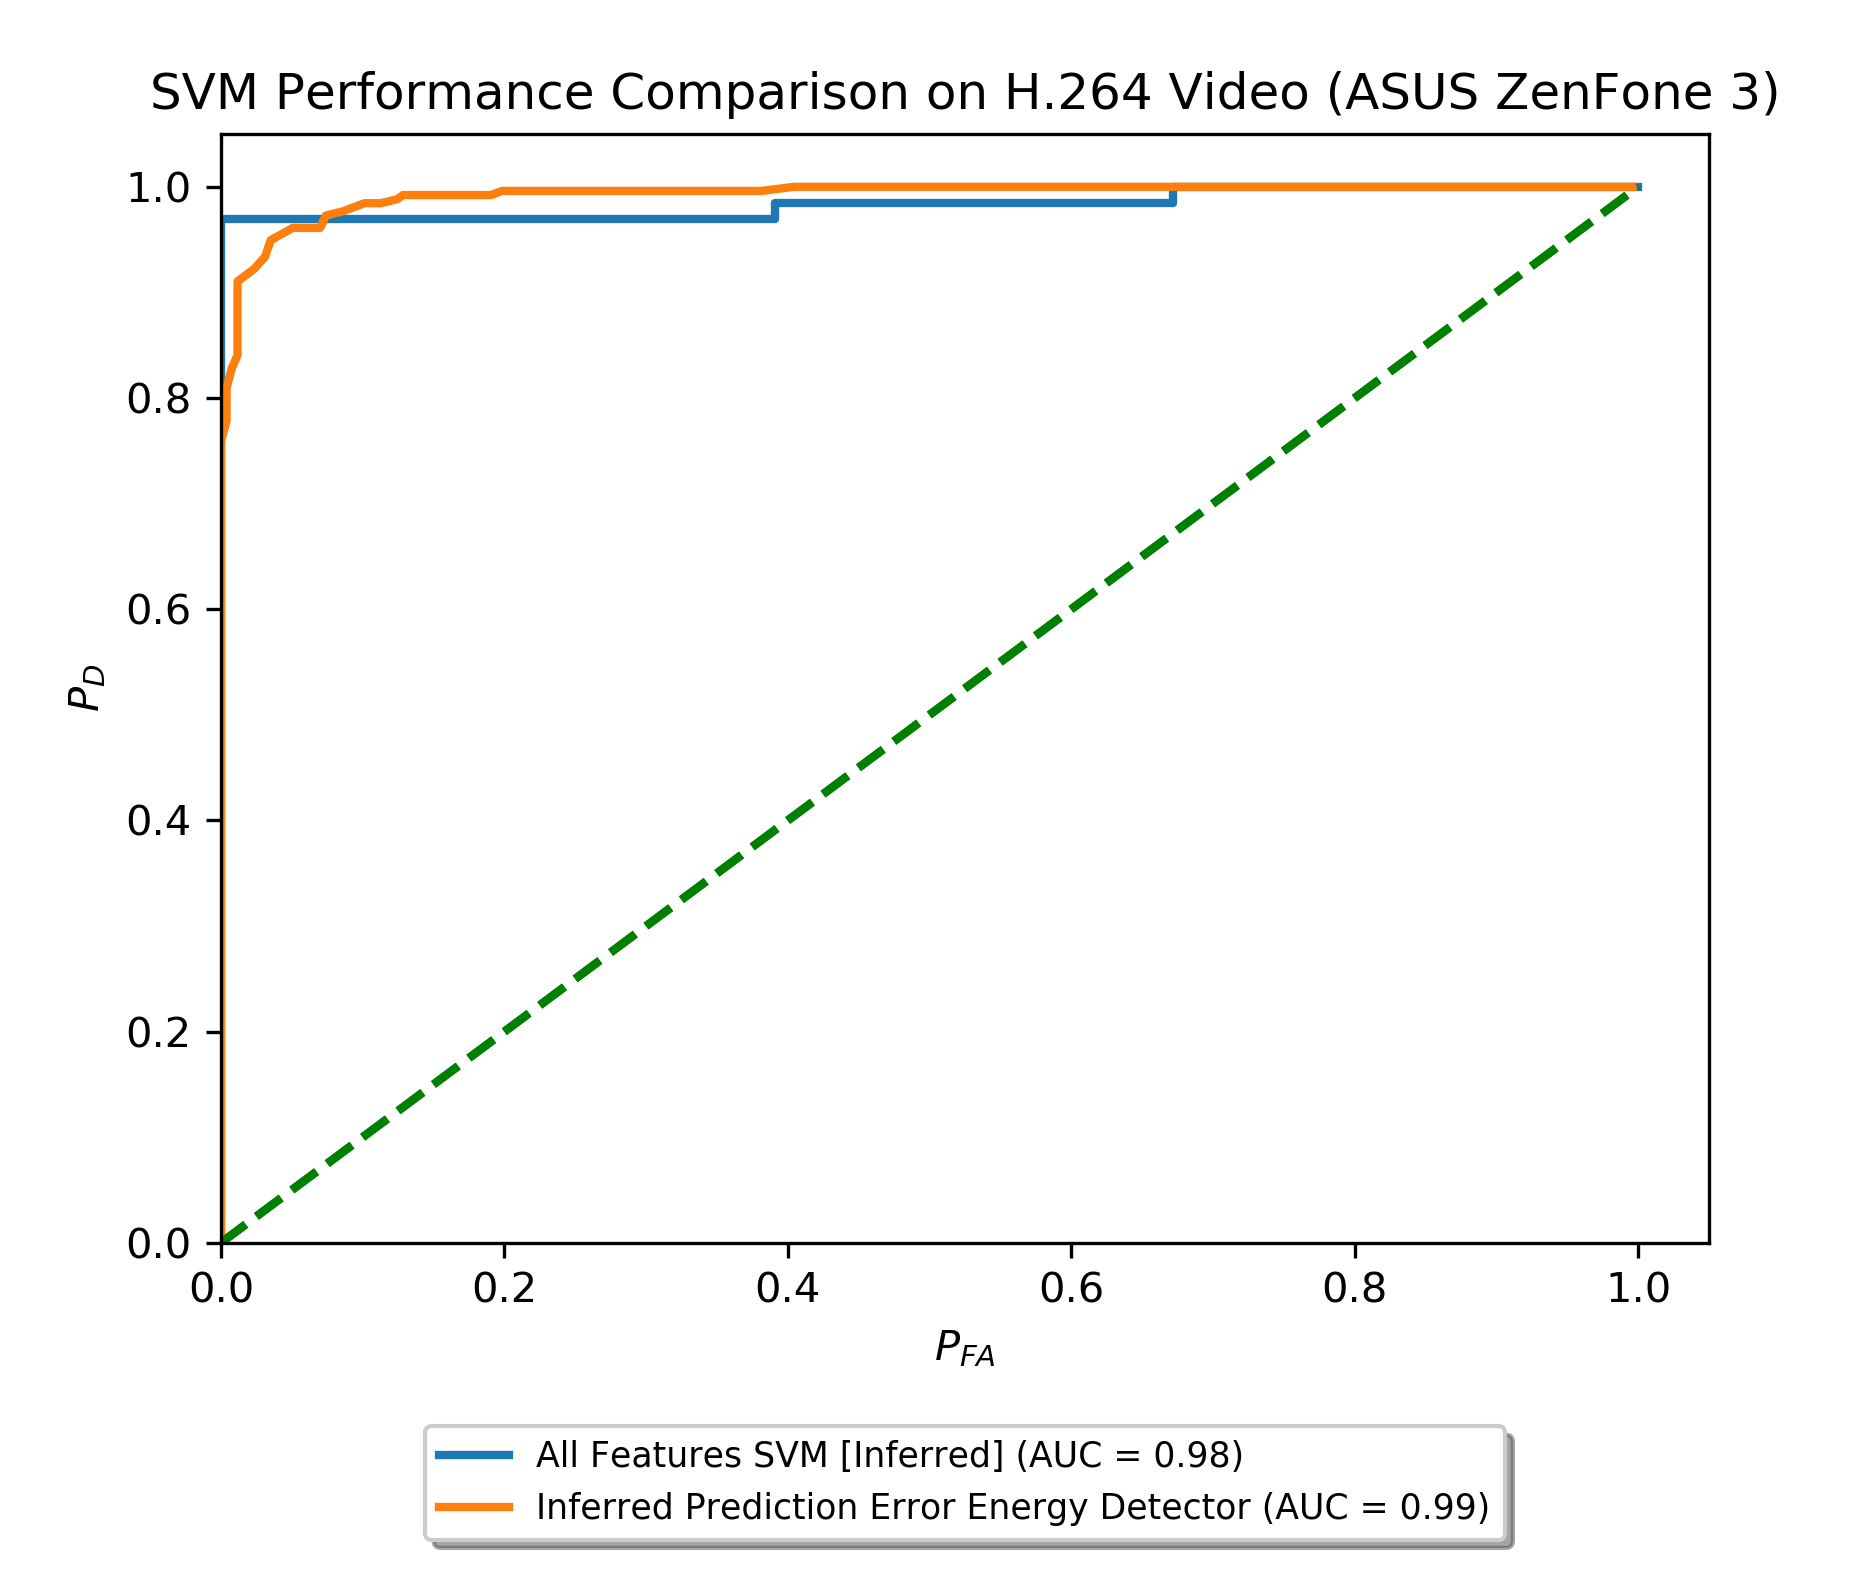
\includegraphics[width=0.7\linewidth]{ExperimentalResults/svm_perror_compare_roc.png}}
\caption{ROC Curves for Inferred Prediction Error Energy Detector and SVM on One Camera Model}
\label{svmrocASUS}
\end{figure}

As the detection rates for the fingerprint energy detector are already above 90\% for low false alarm rates, the relative magnitude of improvement when adding the SVM is less than when changing the prediction error extraction methodology. However, there is a significant improvement at false alarm rates under 10\%. The SVM detector is able to hold above 95\% accuracy at a 0\% false alarm rate. This suggests that some of the frame deleted videos do not have enough statistical differences from genuine videos to be classified as having frames removed from them. The videos in question may have low motion or content such that the fingerprint signal does not express itself in a detectable manner.

\section{Multiple Camera Models}

In order to obtain a better estimate of real world detector performance, we tested the effects of our proposed inferred prediction error extraction method using the entire dataset. We constructed ROC curves for detectors derived from both prediction error extraction methods. The resulting ROC curves can be seen in Fig. ~\ref{perrorExtractFullDS}

\begin{figure}[htbp]
\centerline{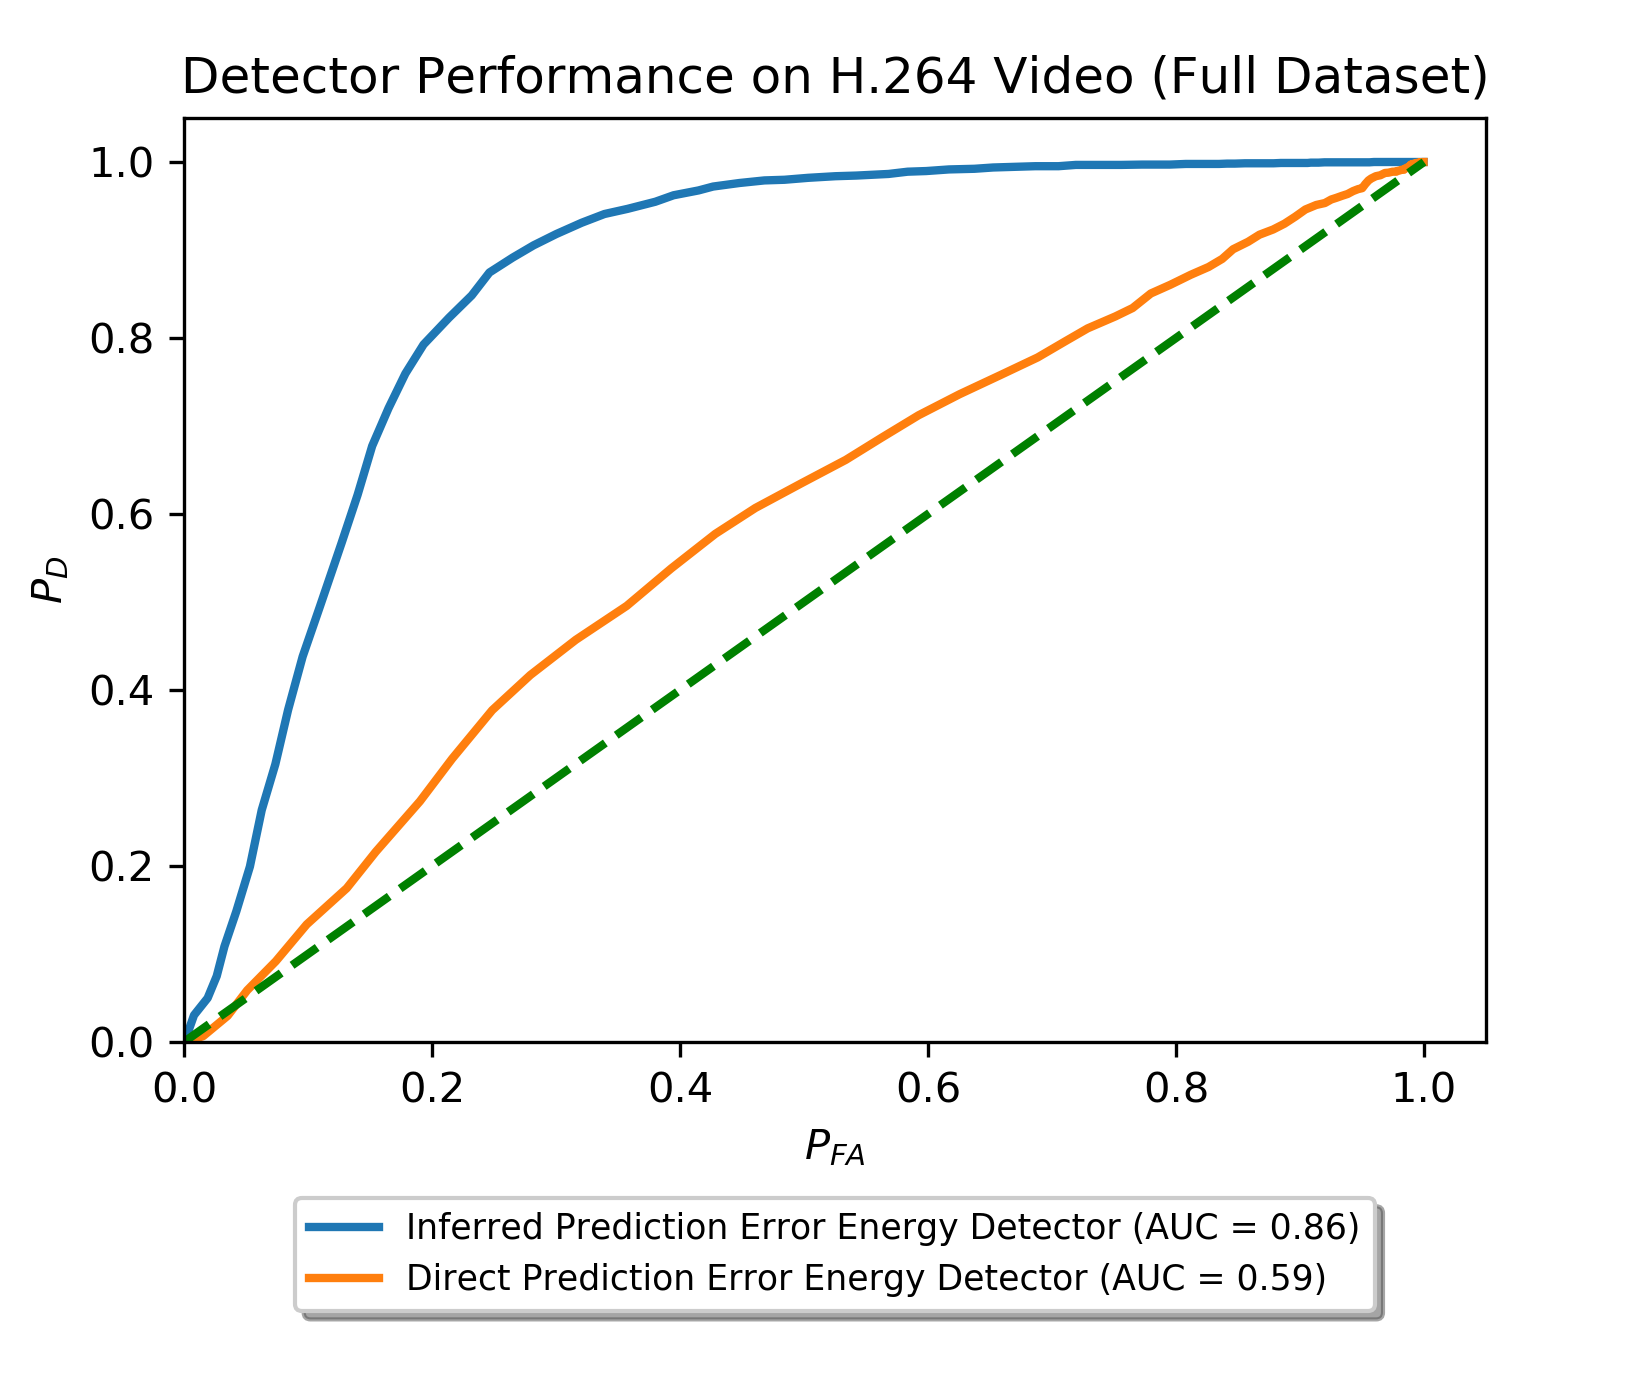
\includegraphics[width=0.7\linewidth]{ExperimentalResults/new_perror_extract_roc_full_ds.png}}
\caption{ROC Curves for Fingerprint Energy Detector Obtained by Using Different Prediction Error Extraction Methods on Multiple Camera Models}
\label{perrorExtractFullDS}
\end{figure} 

It is obvious that the results obtained when testing solely on the ASUS ZenFone 3 were the best case scenarios for both prediction error extraction methods. In fact, using the direct prediction error extraction method from prior research does not yield much better detector performance than random chance. While not optimal, our proposed prediction error extractor provides a much cleaner separability of the data, even when confronted with a wide variety of videos. Without using the SVM, we are able to raise the probability of detection from 15\% to over 60\% at a 10\% false alarm rate.

Before we tested the effects of our expanded feature vector and SVM on the entire dataset, we tuned the SVM to have optimal hyperparameters. We tuned both the penalty of the error term (C) and the size of gaussian used in the radial basis kernel (Gamma). We performed a grid search first in the log-scale to determine their optimal order of magnitude.

\begin{figure}[htbp]%
  \centering
  \subfloat[Log Scale Search for SVM Hyperparameters]{{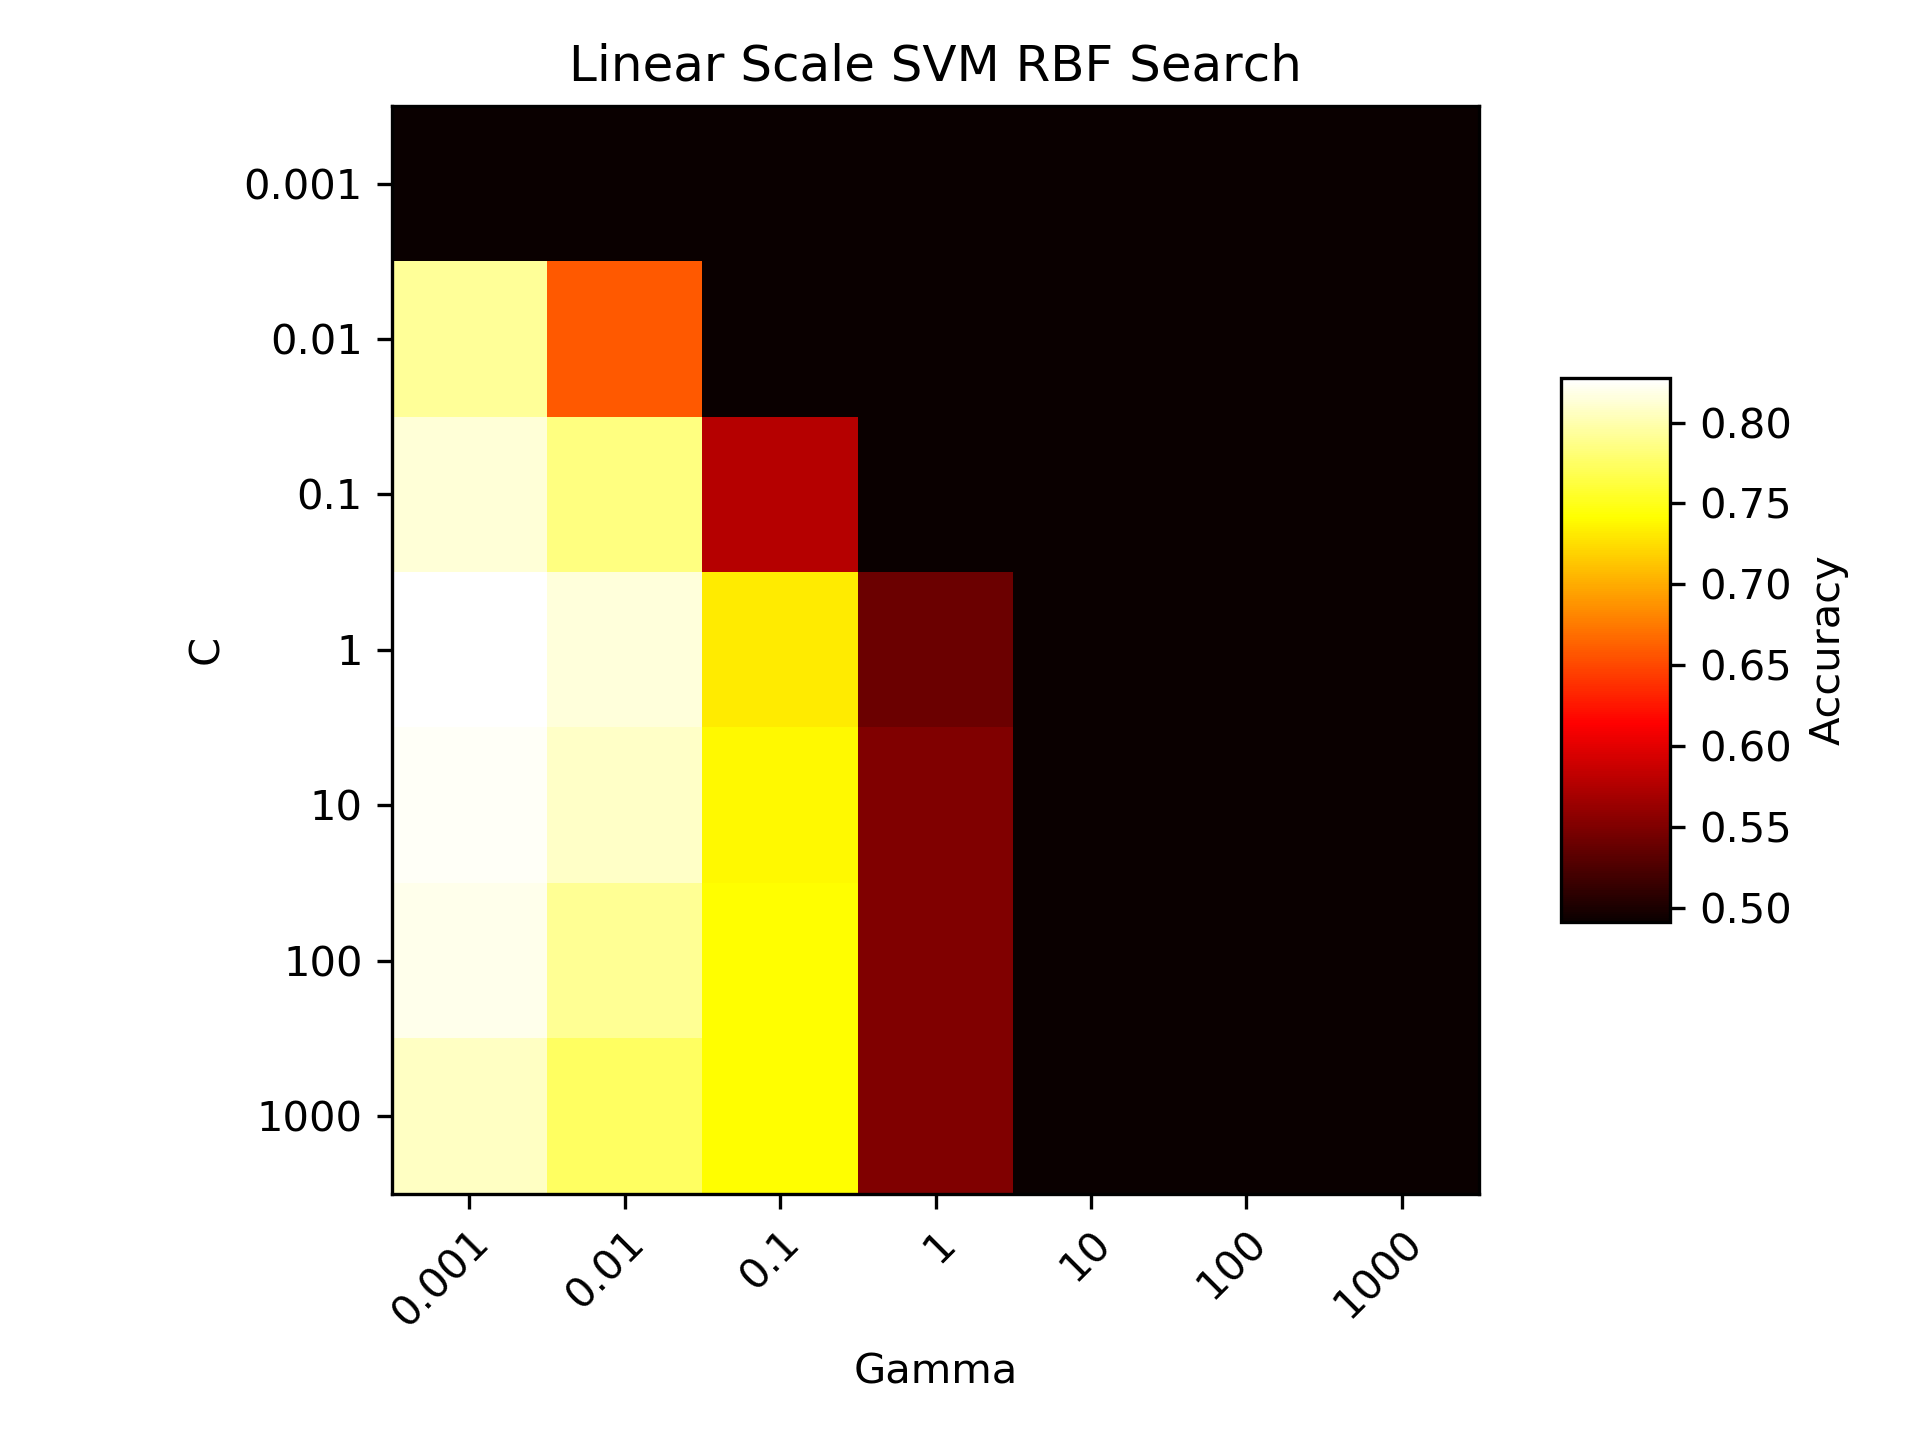
\includegraphics[height=5cm]{ExperimentalResults/log_scale_rbf_search.png}}}%
  \qquad
  \subfloat[Linear Scale Search for SVM Hyperparameters]{{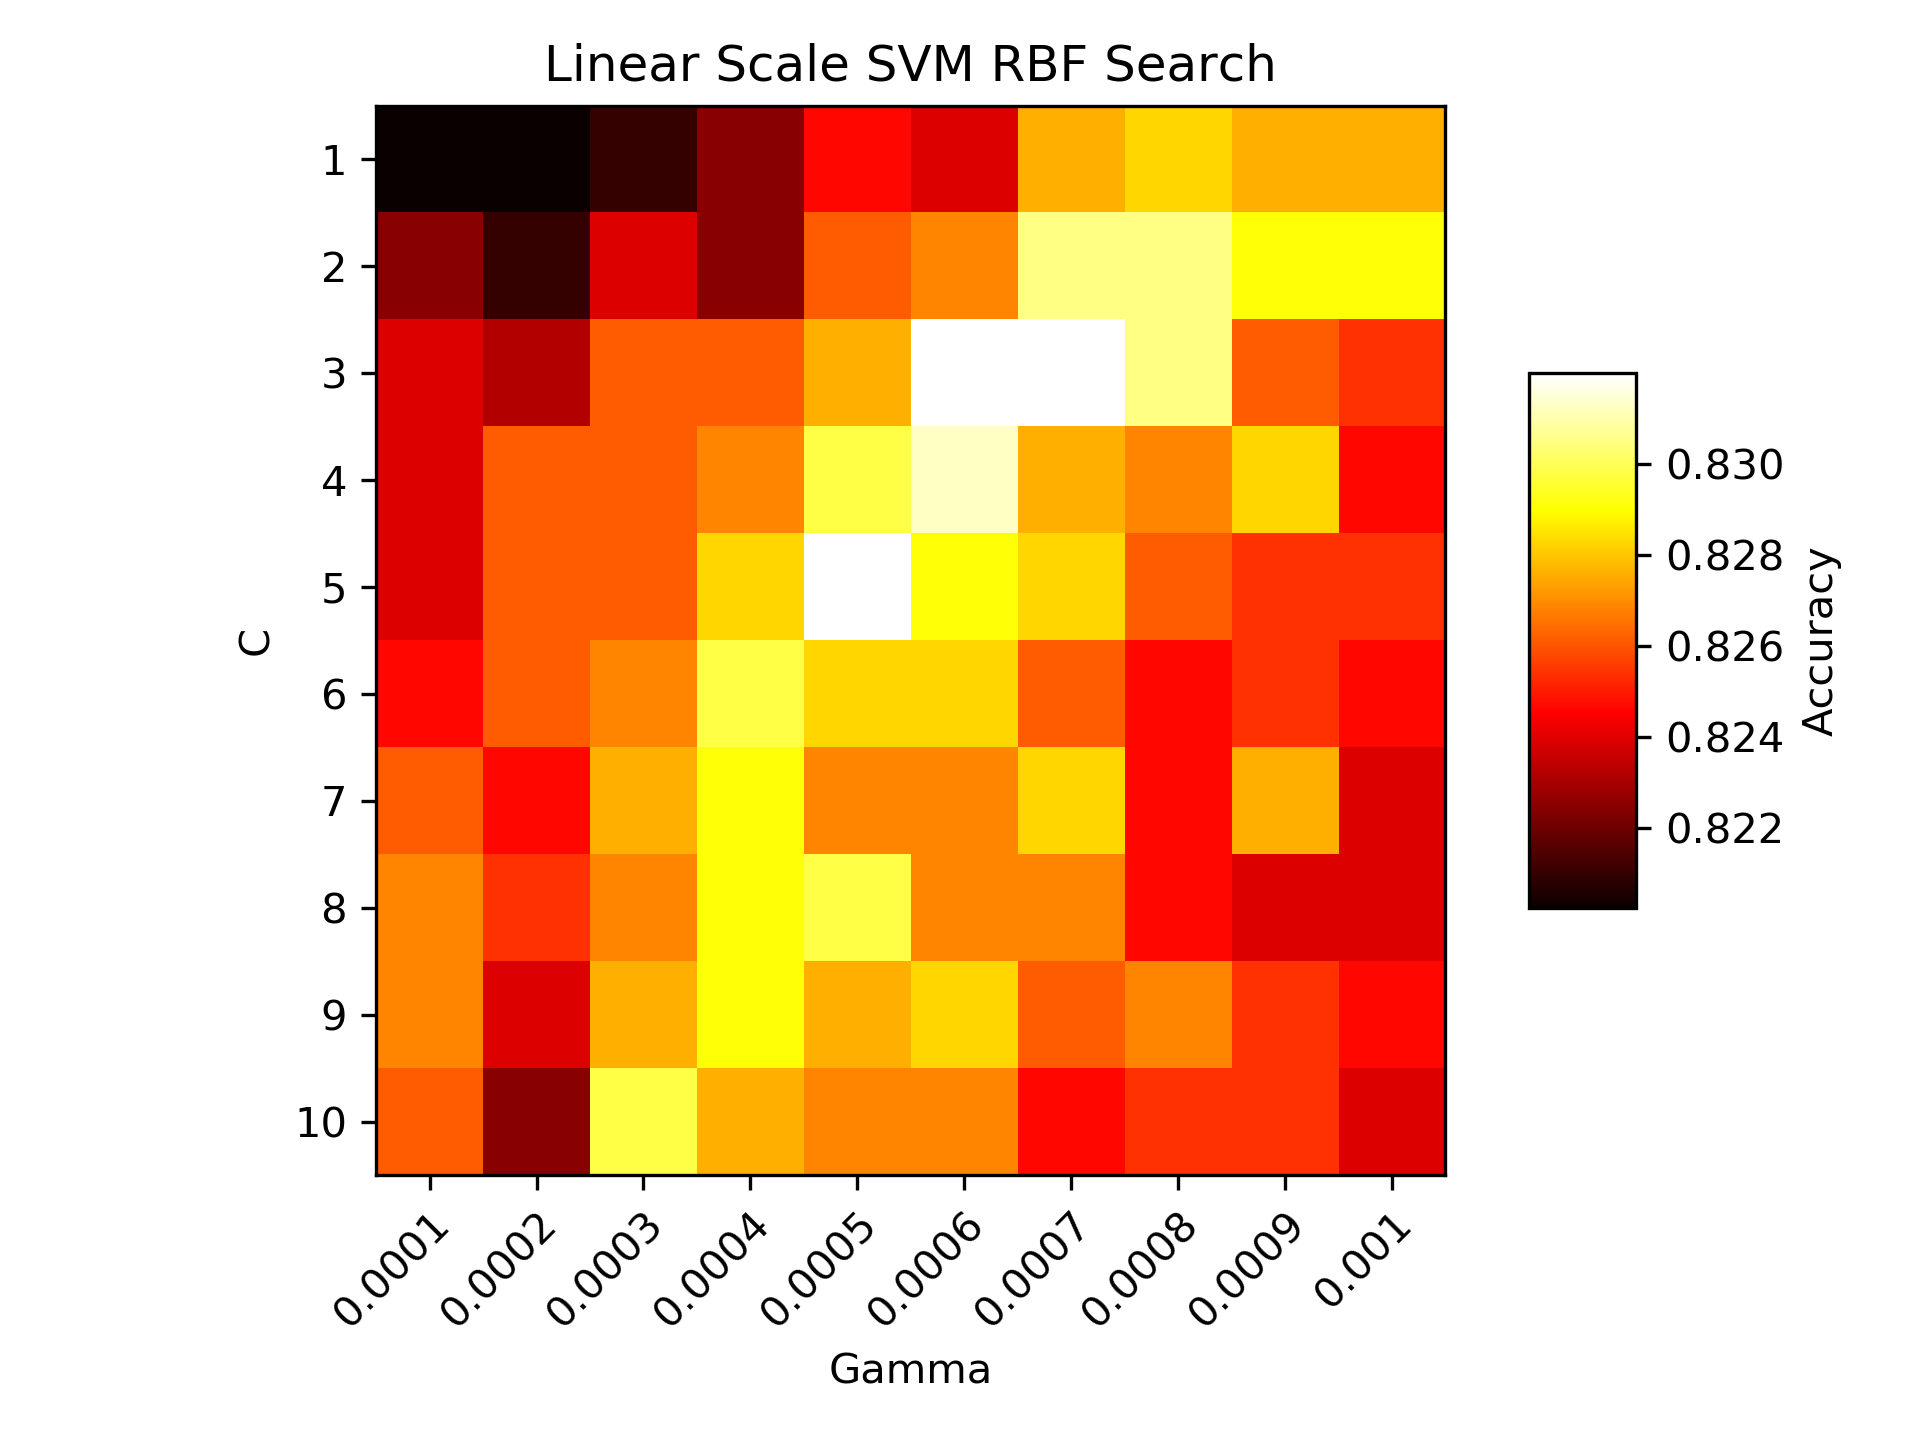
\includegraphics[height=5cm]{ExperimentalResults/lin_scale_rbf_search.png}}}%
\caption{Search for Optimal SVM Hyperparameters on (a) Log Scale and (b) Linear Scale}%
\label{svmparameters}%
\end{figure}

After determining the optimal order of magnitude for both of the hyperparameters, we performed a second grid search, but on a linear scale to find the set of optimal parameters. Fig ~\ref{svmparameters} shows the results of both the log and linear scale grid searches. We chose to use $C = 5$ and $Gamma = 0.0005$ for our SVM. As we did previously, we split our entire dataset into training and testing sets to evaluate the SVM, where the testing set consisted of a quarter of the data. The dataset was shuffled prior to splitting so that a sampling of all camera models would be included in the testing set. Fig. ~\ref{fullDSSVM} shows the ROC curves for the fingerprint energy detectors for both the direct and inferred prediction error extraction methods as well as SVMs.

\begin{figure}[htbp]
\centerline{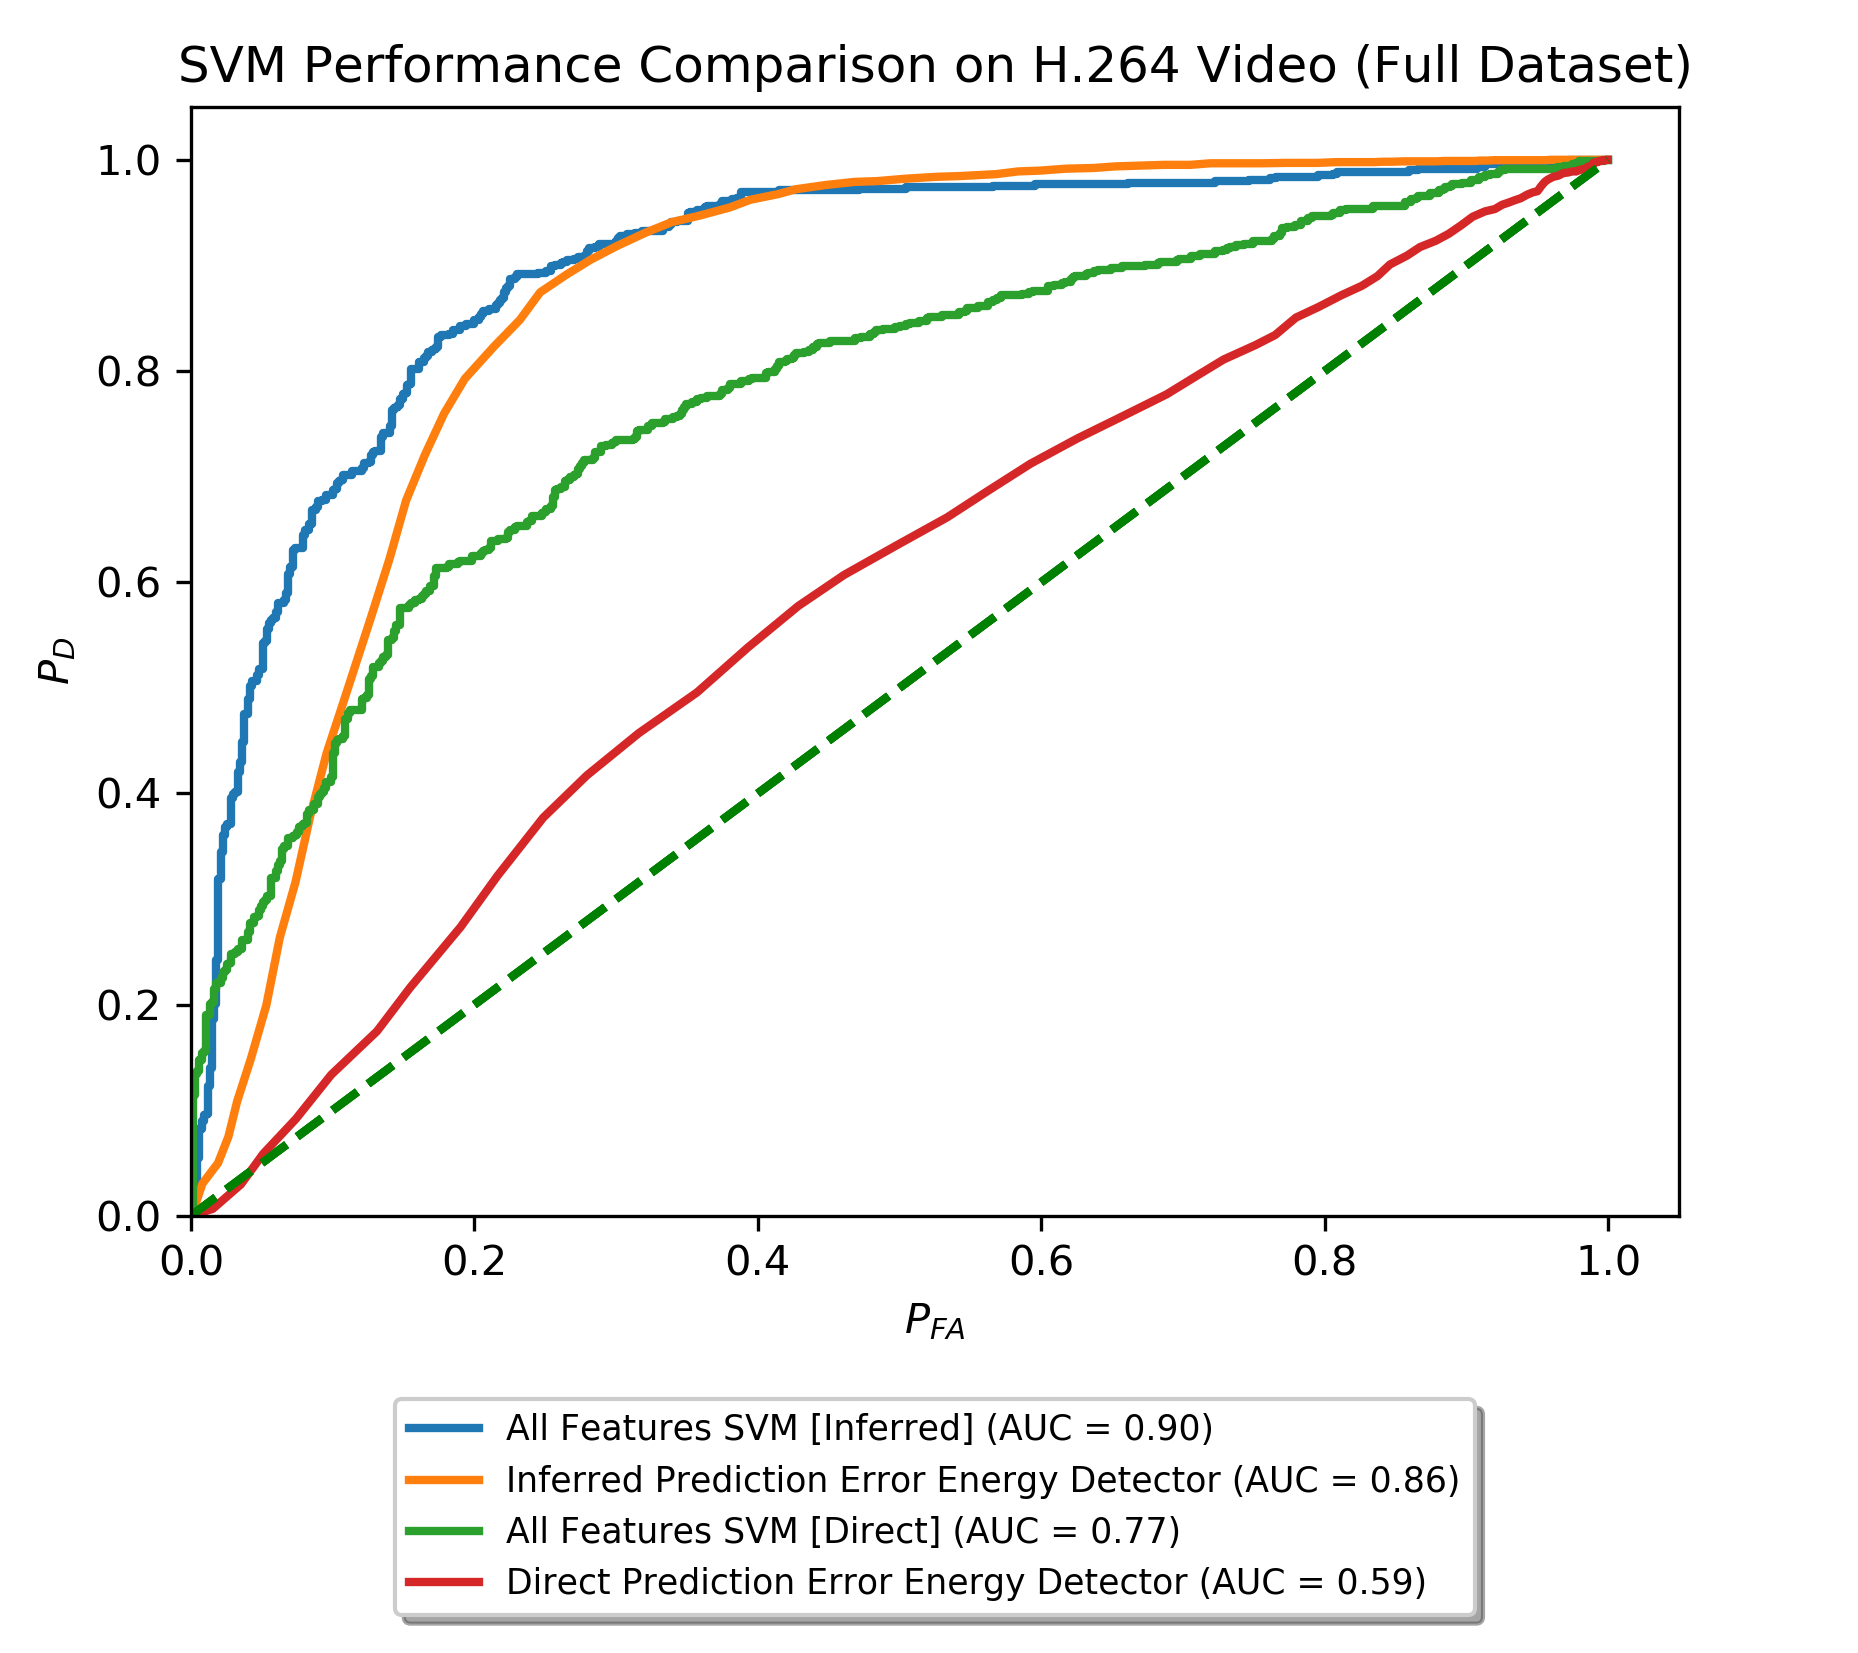
\includegraphics[width=0.7\linewidth]{ExperimentalResults/full_ds_compare_roc.png}}
\caption{ROC Curves for Various Detection Methods on Data from Multiple Camera Models}
\label{fullDSSVM}
\end{figure}

Using our proposed feature vector and SVM with the direct prediction error extraction method allows for some discrimination between the classes. However, the overall detector performance is still less than that of the fingerprint energy detector using our proposed inferred prediction error extraction methodology. Using our proposed feature vector and SVM with our proposed inferred prediction error extraction methodology yields the best detector performance in this scenario, particularly at low false alarm rates. At a 10\% false alarm rate, our combined detector yields an almost 80\% probability of detection.

\section{Additional Work}

As we have shown, our proposed detector is able to distinguish between genuine videos and videos with frame deletion with a reasonable level of accuracy. Indeed, it is also more effective than previously formulated motion vector based detectors, particularly those formulated for use on MPEG-2. However, this is only in a fairly limited scenario. Many videos, especially those shared on social media, are often recompressed, even without having frames removed from them. We tested our proposed detector with a three class classification problem. Given a feature vector $\bm{x}$, it belongs to one of three classes:
\begin{equation}
\begin{aligned}
  C_{0} &: \bm{x} \text{ resulted from a genuine video that has not had frames removed from it.} \\
  C_{1} &: \bm{x} \text{ resulted from an altered video which has had frames removed from it.} \\
  C_{2} &: \bm{x} \text{ resulted from a video that has been recompressed without having frames removed.}
\end{aligned}
\end{equation}

To test this, we created a third set of videos for the ASUS ZenFone 3, where each unaltered video in the dataset was recompressed. Thus we had a dataset of 257 videos for each class. We trained our SVM using the same training and testing data ratio as above, and found optimal parameters for this problem. We tabulated our results into the confusion matrix in Fig. ~\ref{normalcm}.

\begin{figure}[htbp]
\centerline{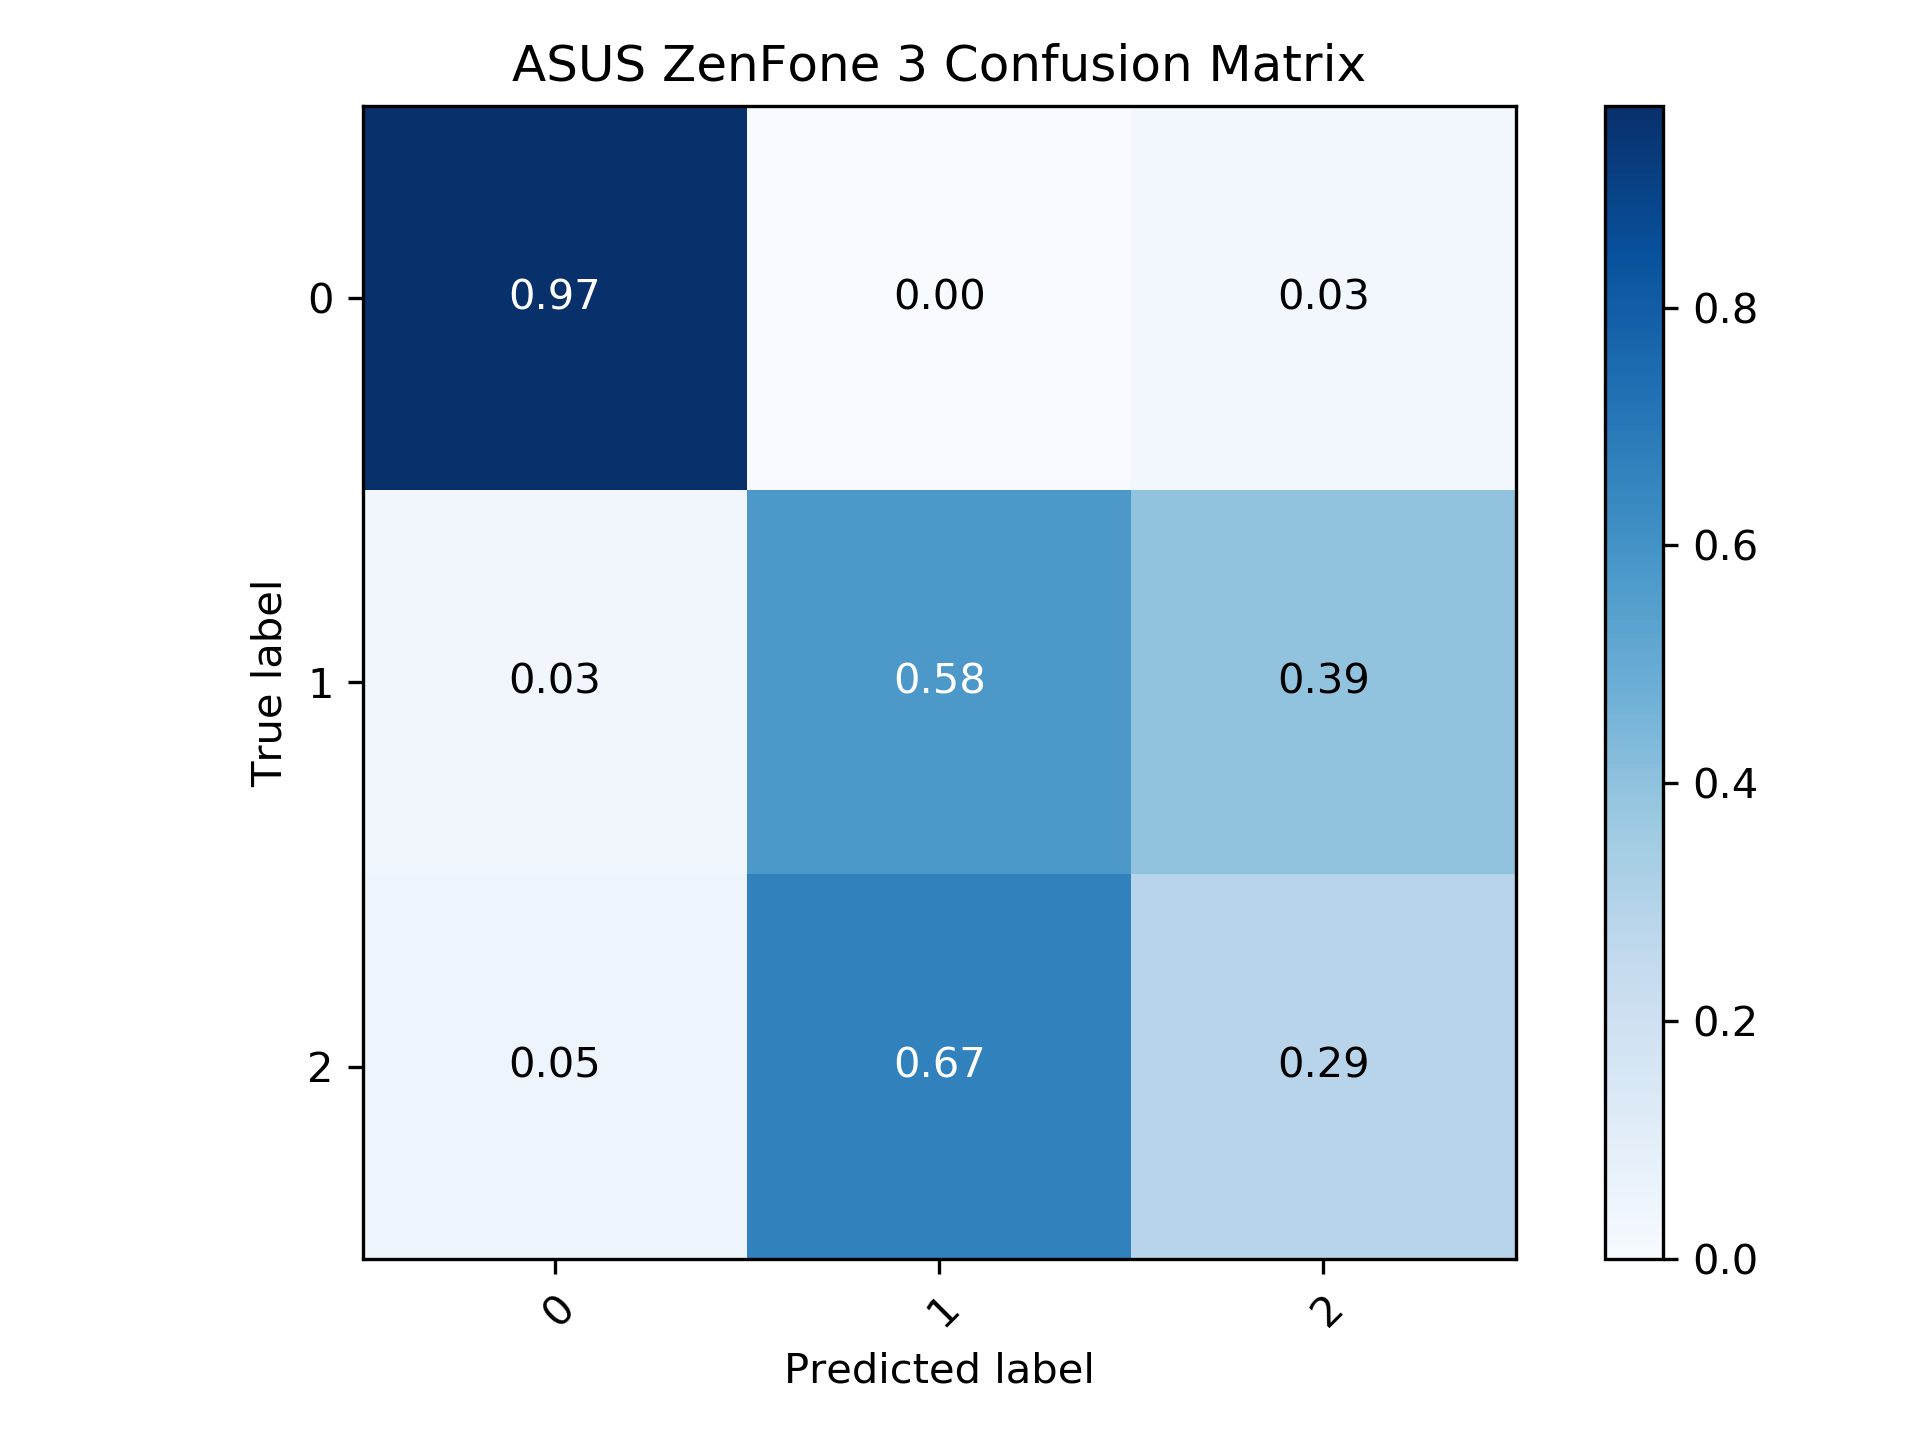
\includegraphics[width=0.7\linewidth]{ExperimentalResults/regular_cm.png}}
\caption{Confusion Matrix for Three Class Classification}
\label{normalcm}
\end{figure}

From this confusion matrix, it becomes clear that more work is needed on our proposed detector. We are able to very easily distinguish whether videos have been recompressed or not, but it is a much more difficult problem to pinpoint the differences between videos that have had frames removed and videos that have only been recompressed. Additional work is needed to make an explicit detector for this scenario. Systems that can learn complex spacial relationships, like Convolutional Neural Networks may be able to help. 

It is possible to tune our proposed detector slightly to increase the overall accuracy of the system. If we scale our data to have zero mean and unit variance on a feature by feature basis, we can trade some accuracy in the genuine class for better distinction between videos with frame deletion and recompressed videos. Fig. ~\ref{scaledcm} shows that we can now detect videos with frame deletion and recompressed videos with just under 60\% accuracy. This puts our overall system accuracy at just under 70\%. While this is a far cry from the over 95\% accuracy on the same camera model with only two classes, it shows that finding differences between videos with frame deletion and recompressed videos is possible.

\begin{figure}[htbp]
\centerline{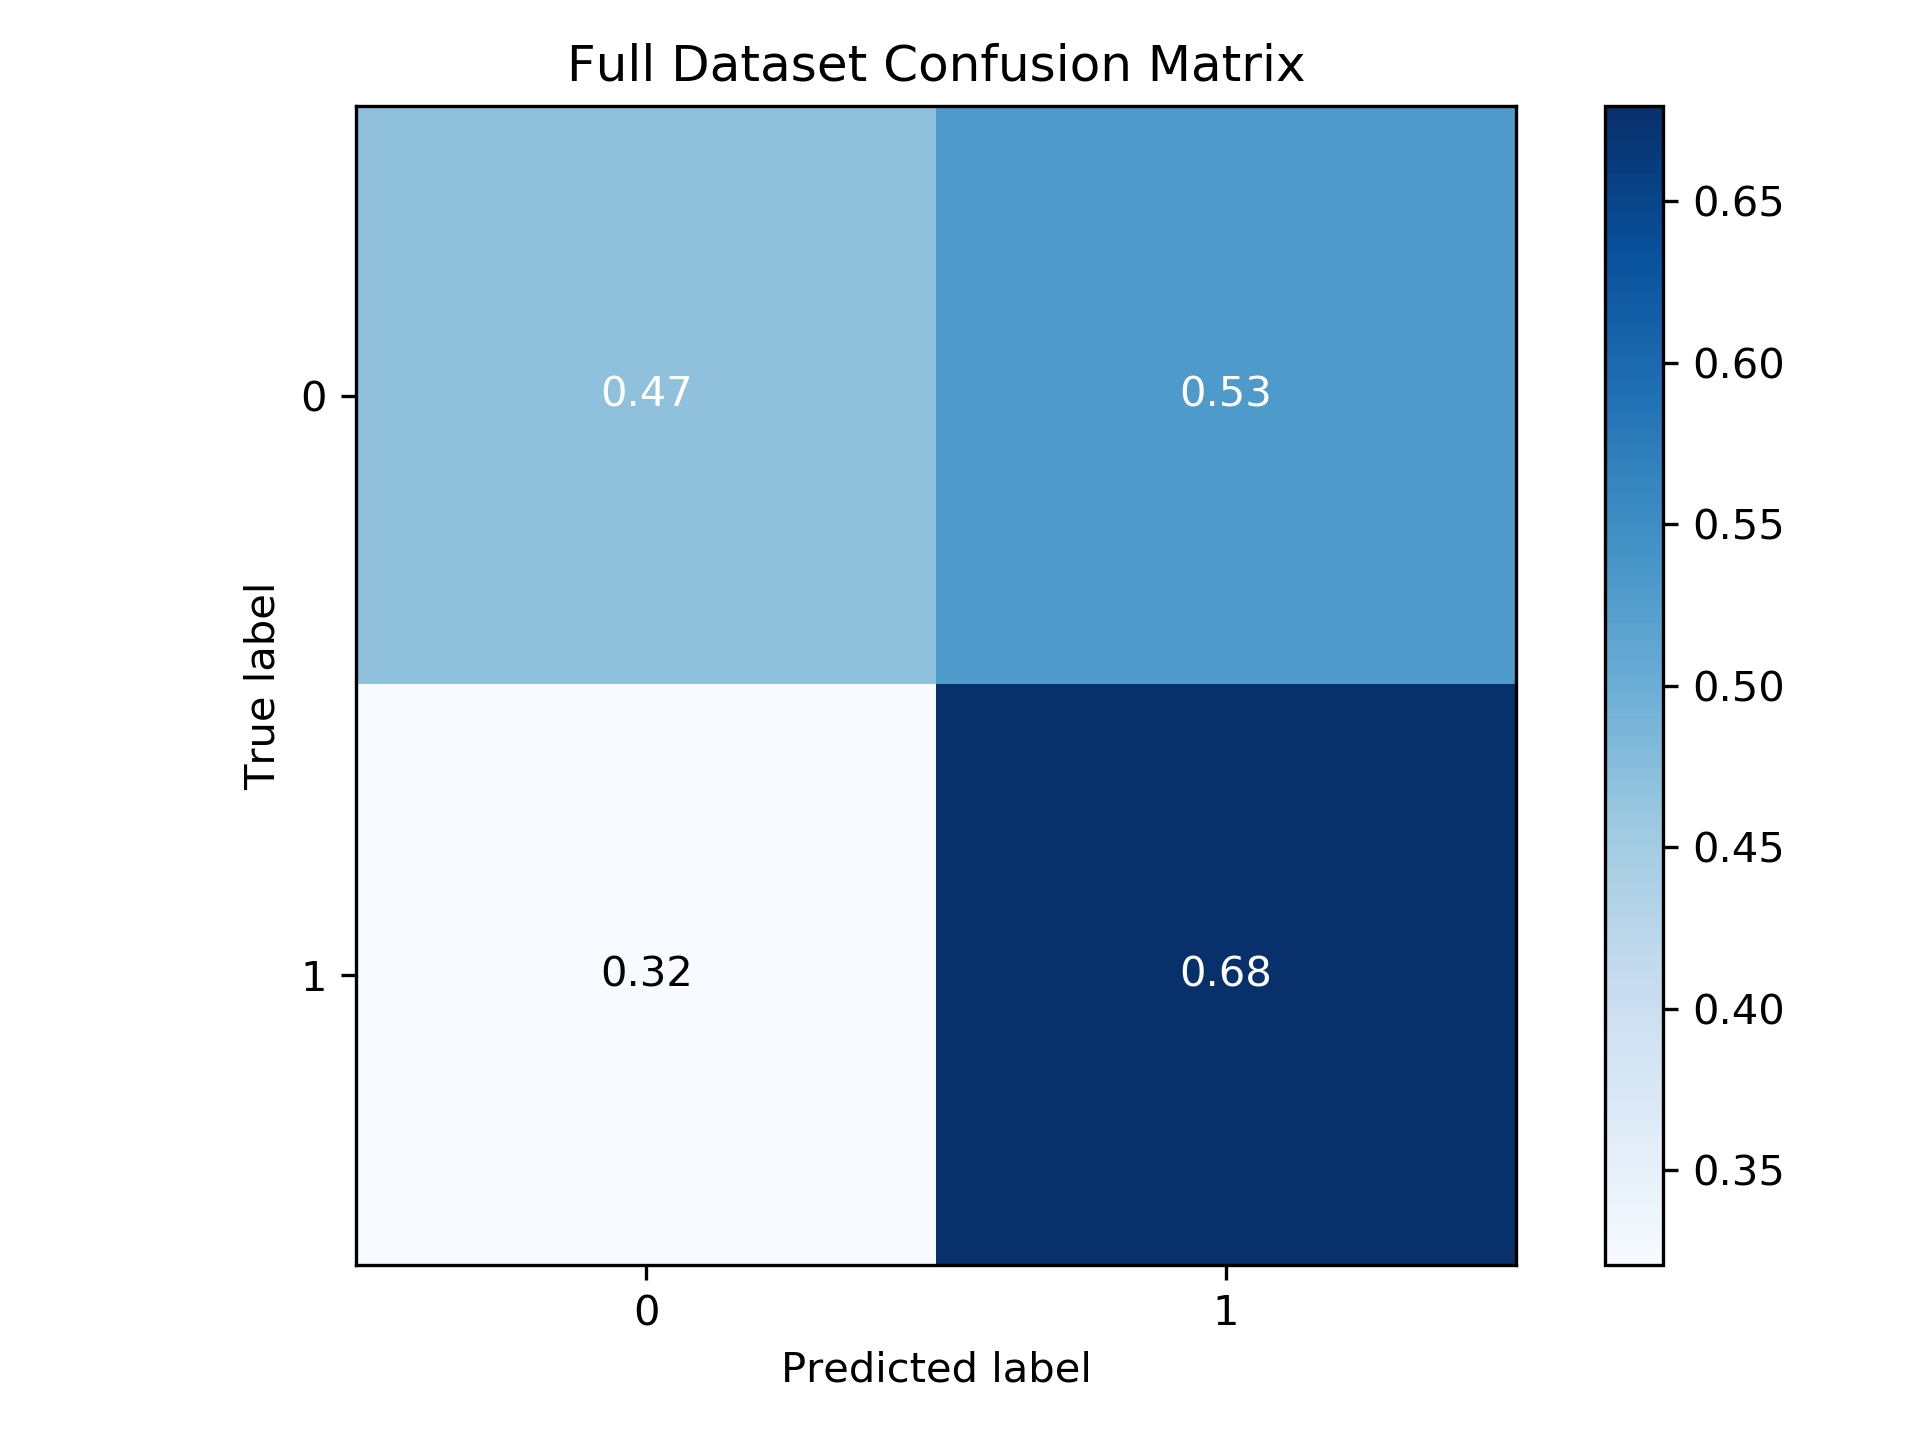
\includegraphics[width=0.7\linewidth]{ExperimentalResults/scaled_cm.png}}
\caption{Confusion Matrix for Three Class Classification using Scaled Data}
\label{scaledcm}
\end{figure}
\chapter{Conclusion}

In this thesis, we have proposed new methods for extracting fingerprints used in detecting frame deletion in modern video as well as an expanded classification framework for more robust classification on real world data. To do this, we first examined previous work on detecting frame deletion in MPEG-2.  We performed an experiment to show that the methodology used for detecting frame deletion in MPEG-2 resulted in detection rates below those obtained in the original research for MPEG-2, and found that due to the differences in motion compensation and estimation found in H.264, an expanded model for the fingerprint signal was needed. We then used this model to alter the prediction error extraction technique to infer the source frame of all macroblocks for every P-frame in the video. Using this inferred prediction error, we were able to isolate the fingerprint signal in an H.264 video. Additionally, we proposed using autoregressive models and additional features to capture statistical variations between videos, and thus shape the decision surface of a Support Vector Machine classifier to be independent of the amount of motion in a video or its scene content.

Through a series of experiments we have evaluated the performance of our proposed prediction error extraction methodology and proposed feature set independently. Our results show that both our proposed prediction error extraction methodology and feature set yield increases to the probability of detecting frame deletion in H.264, particularly at low false alarm rates. This was verified on a diverse set of video captured from multiple camera models and devices. Using both of these techniques together yield an almost 80\% probability of detection at a 10\% false alarm rate, while the methodology proposed for use on MPEG-2 video was unable to accurately identify the set of videos with frame deletion. We also considered the effects of introducing recompressed videos to our proposed detector. We showed that while it is difficult to distinguish between videos with frame deletion and recompressed videos, simple data processing can allow our proposed detection methods to begin to identify their differences. As such, additional work can be done to enable this distinction, potentially with new features or the use of more advanced classification techniques.
\end{thesis}

\printbibliography
%\bibliography{references}

%\appendix
%%%
%% This is file `example-a.tex',
%% generated with the docstrip utility.
%%
%% The original source files were:
%%
%% drexel-thesis.dtx  (with options: `example-appendix')
%% 
%% This is a generated file.
%% 
%% Copyright (C) 2010 W. Trevor King
%% 
%% This file may be distributed and/or modified under the conditions of
%% the LaTeX Project Public License, either version 1.3 of this license
%% or (at your option) any later version.  The latest version of this
%% license is in:
%% 
%%    http://www.latex-project.org/lppl.txt
%% 
%% and version 1.3 or later is part of all distributions of LaTeX version
%% 2003/06/01 or later.
%% 
\chapter{Some Appendix Heading}
\Blindtext[5]
\chapter{Another Appendix Heading}
\Blindtext[5]
\endinput
%%
%% End of file `example-a.tex'.


%\begin{vita}
%\Blindtext[3]
%\end{vita}

\end{document}
\endinput
%%
%% End of file `example.tex'.
